\input{../header.tex}
\usepackage{etoolbox}
\usepackage{placeins}
\usepackage{tikz}
\usepackage[T1]{fontenc}
\usepackage{amsmath, amssymb}
\usetikzlibrary{arrows.meta}

\usetikzlibrary{decorations.pathreplacing}
\usepackage[dvipsnames]{xcolor}
\usetikzlibrary{trees}
\usepackage{algorithm}
\usepackage{algpseudocode}
\usepackage{fancyhdr}
% Define colors
\definecolor{javared}{rgb}{0.6,0,0}
\definecolor{javagreen}{rgb}{0.25,0.5,0.35}
\definecolor{javapurple}{rgb}{0.5,0,0.35}
\definecolor{javadocblue}{rgb}{0.25,0.35,0.75}
\definecolor{pythonblue}{rgb}{0,0,0.6}
\definecolor{pythongreen}{rgb}{0,0.5,0}
\definecolor{pythonred}{rgb}{0.6,0,0}
\definecolor{pythongray}{rgb}{0.5,0.5,0.5}

% Java listing style
\lstdefinestyle{javastyle}{
    language=Java,
    basicstyle=\ttfamily\small,
    keywordstyle=\color{javapurple}\bfseries,
    stringstyle=\color{javared},
    commentstyle=\color{javagreen}\itshape,
    morecomment=[s][\color{javadocblue}]{/**}{*/},
    numbers=left,
    numberstyle=\tiny\color{gray},
    numbersep=8pt,
    tabsize=4,
    showspaces=false,
    showstringspaces=false,
    breaklines=true,
    frame=single,
    rulecolor=\color{black},
    backgroundcolor=\color{white},
    captionpos=b,
    xleftmargin=2em,
    framexleftmargin=1.5em
}

% Python listing style
\lstdefinestyle{pythonstyle}{
    language=Python,
    basicstyle=\ttfamily\small,
    keywordstyle=\color{pythonblue}\bfseries,
    stringstyle=\color{pythonred},
    commentstyle=\color{pythongray}\itshape,
    numbers=left,
    numberstyle=\tiny\color{gray},
    numbersep=8pt,
    tabsize=4,
    showspaces=false,
    showstringspaces=false,
    breaklines=true,
    frame=single,
    rulecolor=\color{black},
    backgroundcolor=\color{white},
    captionpos=b,
    xleftmargin=2em,
    framexleftmargin=1.5em,
    morekeywords={self,True,False,None,as,with}
}


\newcommand{\mcqlist}[1]{%
  \begin{enumerate}[label=(\Alph*), itemsep=0.5em]
    \def\do##1{\item ##1}
    \docsvlist{#1}
  \end{enumerate}
}

% Version number 
\newcommand{\versionNumber}{1.0.3}
\newcommand{\releaseDate}{19.12.2025}


\ShowWarningtrue

\usepackage{listings}
\usepackage{array}
\lstset{upquote=true,basicstyle=\fontencoding{T1}\selectfont\ttfamily}

\newcolumntype{C}[1]{>{\centering\let\newline\\\arraybackslash\hspace{0pt}}m{#1}}

% 2. Setup the footer
\pagestyle{fancy}
\fancyhf{} % Clear current headers/footers
\renewcommand{\headrulewidth}{0pt} % Remove header line if you don't want it

% Keep page number in center, add version on the right
\fancyfoot[C]{\thepage}
\fancyfoot[L]{\small  v\versionNumber\ -- \releaseDate}

\begin{document}

    % Change the following values to true to show the solutions or/and the hints
    \ShowSolutiontrue
    \ShowConseiltrue
    % \ShowWarningtrue
    \titre
    \cours{Banque des questions}


Ce document a été conçu afin de vous servir de support additionnel en plus des slides du cours et des exercices. Les questions n'ont pas fait l'objet du contrôle strict que nous appliquons pour la préparation des ressources documentaires. \newline 

Le temps indiqué (\faClock) est à titre indicatif. \newline 

\section{Architecture et Numération}


\begin{Exercice}[10 minutes]\textbf{Sean}

Dans cet exercice nous aimerions que le processeur calcule et enregistre le produit de 3 fois $10_{10}$ ($00001010_2$) dans le registre 11. Le program counter (PC) commence à \textbf{00000100} et les registres sont initialisés comme suit:

\begin{center}
\begin{tabular}{|c|l|}
\hline
\textbf{Registre} & \textbf{Valeur} \\
\hline
00 & 00001010 \\ \hline
01 & 00000000 \\ \hline
10 & 00000000 \\ \hline
11 & 00000000 \\ 
\hline
\end{tabular}
\end{center}

Les opérations disponibles sont:

\begin{center}
\begin{tabular}{|c|c|}
\hline
\textbf{Numéro} & \textbf{Instruction} \\
\hline
00 & MOV \\ \hline
01 & XOR \\ \hline
10 & ADD \\ \hline
11 & SUB \\ 
\hline
\end{tabular}
\end{center}

\bigskip % Creates vertical space, equivalent to Typst's \ \

% --- Part a ---
\noindent % Prevents indentation
\textbf{a.} Complétez le tableau ci-dessous avec les instructions en binaire nécessaires pour effectuer cette tâche.

\begin{center}
\begin{tabular}{|l|l|}
\hline
\textbf{Adresse} & \textbf{Valeur} \\
\hline
00000100 & \\ \hline
00000101 & \\ 
\hline
\end{tabular}
\end{center}

\bigskip

% --- Part b ---
\noindent % Prevents indentation
\textbf{b.} Donnez le contenu des registres après l'exécution de la première instruction et après l'exécution de la deuxième instruction.

\begin{center}
\begin{tabular}{|c|l|l|}
\hline
\textbf{Registre} & \textbf{Après 1ère instruction} & \textbf{Après 2ème instruction} \\
\hline
00 & & \\ \hline
01 & & \\ \hline
10 & & \\ \hline
11 & & \\ 
\hline
\end{tabular}
\end{center}

\begin{solution}
\textbf{a.}
\begin{center}
\begin{tabular}{|l|l|}
\hline
\textbf{Adresse} & \textbf{Valeur} \\
\hline
00000100 & 10100000\\ \hline
00000101 & 10110010\\ 
\hline
\end{tabular}
\end{center}

\bigskip

\textbf{b.}

\begin{center}
\begin{tabular}{|c|l|l|}
\hline
\textbf{Registre} & \textbf{Après 1ère instruction} & \textbf{Après 2ème instruction} \\
\hline
00 & 00001010 & 00001010 \\ \hline
01 & 00000000 & 00000000 \\ \hline
10 & 00010100 & 00010100 \\ \hline
11 & 00000000 & 00011110 \\ 
\hline
\end{tabular}
\end{center}

\end{solution}
\end{Exercice}

\begin{Exercice}[15 minutes]\textbf{Sean}
Quel est le résultat de la soustraction hexadécimale suivante en base 16: 694F - 5A3C?

\begin{solution}
0F13
\end{solution}
\end{Exercice}


\begin{Exercice}[10 minutes]\textbf{Aurore}
Selon le modèle de Von Neumann, partant d'un program counter valant 101010 et d'une mémoire contenant les instructions suivantes:
\begin{table}[h]
\centering
\begin{tabular}{|c|c|}
\hline
\textbf{Adresse} & \textbf{Instruction} \\
\hline
101001 & 01000111 \\ \hline
101010 & 01111000 \\ \hline
101011 & 10001101 \\ \hline
101100 & 10010110 \\ 
\hline
\end{tabular}
\end{table}

Dans quel registre le résultat de la prochaine opération va-t-il être stocké?

\mcqlist{00, 01, 10, 11}

\begin{solution}
11
\end{solution}

\end{Exercice}

\begin{Exercice}[10 minutes]\textbf{Aurore} Quel est le résultat de l'opération suivante : $395_{16}$ + $1011101_{2}$?
\mcqlist{$1011_{10}$, $3F2_{16}$, $0011 1110 0011_2$, $1010_2$}

\begin{solution}
$3F2_{16}$
\end{solution}
\end{Exercice}

\begin{Exercice}[10 minutes]\textbf{Maxim} Quelle est la valeur en base 10 de l’opération suivante : $128_9$ - $245_6$?
\mcqlist{9,6,0,3}
\begin{solution}
6
\end{solution}
\end{Exercice}

\begin{Exercice}[10 minutes]\textbf{Maxim}
Convertir le nombre $127_{10}$ en base 8.
\mcqlist{87,177,71,180}
\begin{solution}
$177_8$
\end{solution}
\end{Exercice}

\begin{Exercice}[10 minutes]\textbf{Léa}
Quel est le résultat de l'opération suivante $67_8$ + $110111_2$ en base 10? 
\mcqlist{110, 78, 122, 106}
\begin{solution}
    110
\end{solution}
\end{Exercice}

\begin{Exercice}[10 minutes]\textbf{Léa}
En suivant le modèle de von Neumann, l'Instruction Register (IR) a une valeur de 11000111, les registres contiennent les valeurs suivantes:
\begin{table}[h!]
\centering
\begin{tabular}{|c|c|}
\hline
\textbf{Registre} & \textbf{Valeur} \\ \hline
00 & 00000000 \\  \hline
01 & 00000101 \\  \hline
10 & 00000110 \\  \hline
11 & 00000010 \\ \hline
\end{tabular}
\end{table}

\begin{center}
\begin{tabular}{|c|c|}
\hline
\textbf{Numéro} & \textbf{Valeur} \\ \hline
00 & MOV \\  \hline
01 & XOR \\  \hline
10 & ADD \\  \hline
11 & SUB \\ \hline
\end{tabular}
\end{center}
Quelle est la valeur du résultat de l'opération?
\mcqlist{$00000111_2$, $00001011_2$, $00000011_2$, $00000001_2$}
\begin{solution}
$00000011_2$ est stocké dans le registre 00.
\end{solution}
\end{Exercice}

% \begin{Exercice}[10 minutes]\textbf{Léa}
% Quelle est la valeur du résultat de l'opération?
% \mcqlist{$111_2$, $1011_2$, $011_2$, $0001_2$}
% \end{Exercice}

\begin{Exercice}[10 minutes]\textbf{Reda}
Que représentent les deux premiers bits (partant de gauche) de l'Instruction Register? (exemple: 11001001)?
\mcqlist{L'adresse du registre dans lequel il faudra mettre le résultat,
L'identificateur de l'opération à exécuter,
L'adresse du registre dans lequel est contenue la valeur sur laquelle faire l'opération,
Ils n'ont aucune signification}

\begin{solution}
Option B.
\end{solution}
\end{Exercice}

\begin{Exercice}[10 minutes]\textbf{Reda}
Quel est le résultat de la soustraction $11011001_2$ - $00110110_2$ en base 10?
\begin{solution}
163
\end{solution}
\end{Exercice}

\begin{Exercice}[10 minutes]\textbf{Amina}
Quel est le résultat de l'opération suivante : $1011010_2$ - $1000111_2$?
\mcqlist{$0001111_2$, $0010011_2$, $0100011_2$, $0010101_2$}
\begin{solution}
$0010011_2$
\end{solution}
\end{Exercice}


\begin{Exercice}[10 minutes]\textbf{Amina}
Quel est le résultat en base 10 de l'opération suivante : $47_{10}$ + $DEF_{16}$ ?
\mcqlist{3614, 3478, 3589, 3651}
\begin{solution}
    3614
\end{solution}
\end{Exercice}


\begin{Exercice}[10 minutes]\textbf{Léa}
Écrivez le complément à 2 de $21_{10}$ sur 8 bits:
\mcqlist{1110 1011, 1110 1010, 0001 0101, 0001 0100}

\begin{solution}
Option A. 
\end{solution}
\end{Exercice}


\begin{Exercice}[10 minutes]\textbf{Amina}
Quelle est la représentation du complément à 2 (two complement) de -143 sur 8 bits?

\mcqlist{10010001, 01110001, 01100001, Aucune des réponses n'est correcte}

\begin{solution}
La valeur la plus négative sur 8 bits en complément à deux est $-2^7=-128$. Aucune des réponses n'est correcte.
\end{solution}
\end{Exercice}

\pagebreak
\section{Systèmes d'exploitation et langages de programmation}

\begin{Exercice}[10 minutes]\textbf{Maxim}
Quel est l'avantage principal d'un langage compilé ?
\mcqlist{Plus facile à corriger, Exécution plus rapide, Plus simple à écrire que les autres langages, Indépendant du système d’exploitation}
\begin{solution}
Option B.
\end{solution}
\end{Exercice}

\begin{Exercice}[10 minutes]\textbf{Maxim}
    Quelle est la différence entre un compilateur et un interpréteur ?
    \mcqlist{Le compilateur traduit le code au moment de l’exécution et l’interpréteur traduit le code avant l’exécution,
    Le compilateur traduit le code avant l’exécution et l'interpréteur traduit le code au moment de l’exécution,
    Les deux font exactement la même chose,
    Le compilateur n’est utilisé que pour les systèmes Unix}

    \begin{solution}
        Option B. 
    \end{solution}
\end{Exercice}

\begin{Exercice}[10 minutes]\textbf{Léa}

Voici la visualisation de vos dossiers (exemple: Dans le dossier Cours il y a un dossier Cours\_1):

\begin{figure}[h!]
\begin{tikzpicture}[scale=1.6,
    every node/.style = {draw=black, thick, anchor=west},
    selected/.style = {draw=OliveGreen, fill=green!30},
    file/.style = {draw=blue, fill=cyan!30},
    optional/.style = {dashed, fill=gray!50},
    grow via three points={one child at (0.5,-0.7) and two children at (0.5,-0.7) and (0.5,-1.4)},
    edge from parent path={(\tikzparentnode.south) |- (\tikzchildnode.west)}
]
\node [selected] {\faFolder[regular] /User}
child { 
    node [selected] {\faFolder[regular] /Cours}
    child { 
        node [selected] {\faFolder[regular] /Cours\_1}
        child { 
            node [file] {\faFile[regular] Slides\_1.pdf}
        }
    }
}
child [missing] {}
child [missing] {}
child { 
    node [selected] {\faFolder[regular] /TPs}
    child { 
        node [selected] {\faFolder[regular] /Solutions}
    }
    child { 
        node [file] {\faFile[regular] tp1.py}
    }
    child { 
        node [file] {\faFile[regular] tp1.java}
    }
}
child [missing] {}
child [missing] {}
child [missing] {}
child { 
    node [selected] {\faFolder[regular] /Documents}
}
child { 
    node [selected] {\faFolder[regular] /Photos}
};
\end{tikzpicture}
\end{figure}
\FloatBarrier

Vous ouvrez un terminal et vous êtes dans le dossier TPs, qu'est ce qui va être affiché dans le terminal si vous tapez \texttt{ls} sur un système d'exploitation UNIX (Linux/MacOS) (on écrit tout à la même ligne par souci de concision):

\mcqlist{\texttt{Solutions tp1.py tp1.java}, \texttt{TPs Solutions tp1.py tp1.java}, \texttt{Cours Cours\_1 Slides\_1 TPs Solutions tp1.py tp1.py Photos Documents}, \texttt{tp1.py tp1.java}}

\begin{solution}
Option A. 
\end{solution}
\end{Exercice}

\begin{Exercice}[10 minutes]\textbf{Léa}
Vous êtes toujours dans le dossier TPs et vous voulez aller dans le dossier Solutions, quelle commande tapez vous dans le terminal?
\mcqlist{\texttt{rm Solutions},\texttt{mv Solutions}, \texttt{cd Solutions},\texttt{mkdir Solutions}}
\begin{solution}
Option C. 
\end{solution}
\end{Exercice}

\begin{Exercice}[10 minutes]\textbf{Sean}


Vous vous trouvez dans un dossier qui contient deux sous-dossiers : \faFolder[regular] \textcolor{blue}{python} et \faFolder[regular] \textcolor{blue}{java}.
\begin{itemize}
    \item[$\bullet$] Le dossier \textcolor{blue}{python} contient un unique fichier nommé \textcolor{green}{hello.py}.
    \item[$\bullet$] Le dossier \textcolor{blue}{java} contient un unique fichier nommé \textcolor{green}{hi.java}.
\end{itemize}

\textbf{(a)} Quelle(s) commande(s) devez-vous taper dans le terminal, ouvert depuis le dossier \textbf{parent} de \textcolor{blue}{python}, pour exécuter le programme \textit{hello.py} ? \\ 

\textbf{(b)} Après avoir exécuté les commandes de la question (a), quelles commandes faut-il saisir pour compiler puis exécuter le programme \textit{hi.java} situé dans le dossier \textit{java} ? \\ 

\textbf{(c)} Après avoir exécuté le programme \textit{hi.java}, si vous vous placez dans le dossier \textit{java} et que vous tapez la commande \textbf{ls}, quelle sera la sortie affichée dans le terminal ?

\begin{solution}
\textbf{a.} \texttt{python python/hello.py} \newline 
\textbf{b.} \texttt{javac java/hi.java} ensuite \texttt{java java/hi.javac}. Alternativement, \texttt{javac java/hi.java \&\& java java/hi.javac} \newline 
\textbf{c.} \\
\texttt{hi.javac} \newline \texttt{hi.java}  
\end{solution}
% \vspace{1em}
% \noindent\rule{\textwidth}{0.4pt}

% \subsection{Solution}

% \textbf{(a)}

% \begin{lstlisting}[language=bash]
% cd python
% python hello.py
% \end{lstlisting}

% Alternative en une seule commande :

% \begin{lstlisting}[language=bash]
% python python/hello.py
% \end{lstlisting}

% \noindent{\color{Maroon}\rule{4cm}{2pt}}

% \textbf{(b)}

% \begin{lstlisting}[language=bash]
% cd ..
% cd java
% javac hi.java
% java hi
% \end{lstlisting}

% Alternative si vous êtes toujours dans le dossier parent de python :

% \begin{lstlisting}[language=bash]
% cd java
% javac hi.java
% java hi
% \end{lstlisting}

% \noindent{\color{Maroon}\rule{4cm}{2pt}}

% \textbf{(c)}

% La sortie affichée sera :

% \begin{lstlisting}
% hi.java
% hi.class
% \end{lstlisting}

\end{Exercice}


\begin{Exercice}[10 minutes]\textbf{Amina}
La commande \texttt{pwd} permet de:
\mcqlist{Afficher le chemin absolu du répertoire courant, Supprimer le répertoire courant, Créer un nouveau fichier, Afficher la liste des fichiers dans le répertoire courant.}
\begin{solution}
Option A. 
\end{solution}
\end{Exercice}

\begin{Exercice}[10 minutes]\textbf{Amina}
Parmi ces commandes, laquelle permet de créer un nouveau répertoire ?
\mcqlist{\texttt{ls}, \texttt{cd}, \texttt{mkdir}, \texttt{pwd}}
\begin{solution}
\texttt{mkdir}
\end{solution}
\end{Exercice}

\begin{Exercice}[10 minutes]\textbf{Aurore}
Voici la ligne de commande d'un terminal sur une machine MacOS/Linux (à gauche) et Windows (à droite).

\begin{figure}[h!]
    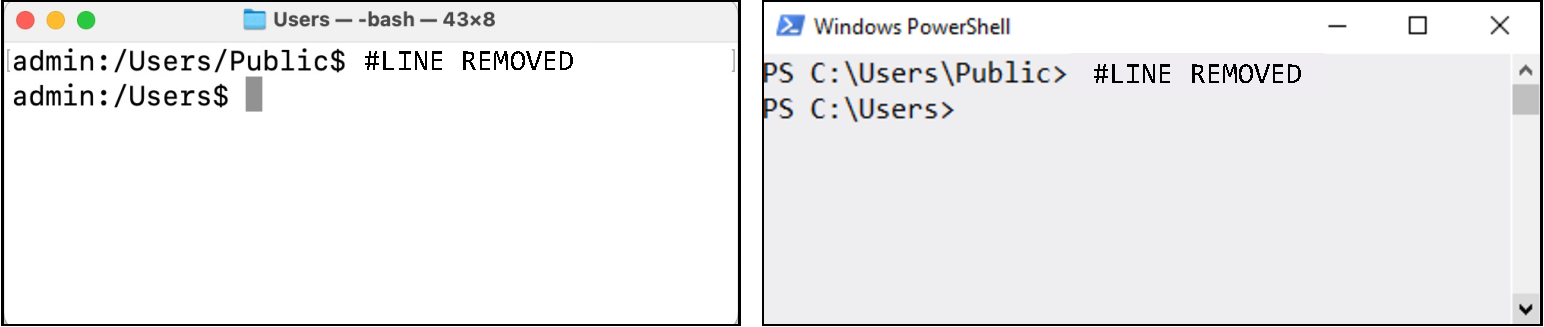
\includegraphics[width = \textwidth]{res/bashq21.pdf}
\end{figure}

Quelle commande a été passée (\#LINE REMOVED)?

\mcqlist{\texttt{dir}, \texttt{cd Users}, \texttt{cd ..}, \texttt{ls}}
\begin{solution}
\texttt{cd ..}
\end{solution}
\end{Exercice}


\begin{Exercice}[10 minutes]\textbf{Aurore}
Laquelle des affirmations suivantes est fausse?
\mcqlist{Un langage compilé est traduit ligne par ligne au moment de l'exécution, 
{En Java, l'étape de compilation et d'interprétation sont séparées}, 
Un langage interprété est plus lent à exécuter, 
Les langages Python et Java nécessitent les deux une traduction en bytecode, 
Toutes les affirmations sont correctes}

\begin{solution}
Option A. 
\end{solution}
\end{Exercice}

\pagebreak
\section{Bases de la programmation}

\begin{Exercice}[10 minutes]\textbf{Maxim}
En Java, que signifie le mot-clé final appliqué à une variable?
\mcqlist{La variable ne peut pas être utilisée dans une boucle,
La variable est constante et ne peut pas changer de valeur, 
 La variable est automatiquement initialisée à zéro, 
 La variable est globale}

 \begin{solution}
Option B. 
 \end{solution}

\end{Exercice}

\begin{Exercice}[10 minutes]\textbf{Maxim}
Si on exécute le code suivant:

\begin{lstlisting}[style=pythonstyle]
x = 7 
if x % 2 == 0: 
   print("pair") 
else: 
   print("impair") 
\end{lstlisting}
Que sera affiché?

\mcqlist{impair, pair, 7, Aucun affichage}

\begin{solution}
Option A. 
\end{solution}
\end{Exercice}

\begin{Exercice}[10 minutes]\textbf{Léa}
Qu'affiche le code suivant écrit en Java?

\begin{lstlisting}[style=javastyle]
int numero_jour = 5;
switch (numero_jour) {
    case 1:                
        System.out.println("Lundi");
        break;
    case 2:
        System.out.println("Mardi");
        break;
    case 3:
        System.out.println("Mercredi");
        break;
    case 4:
        System.out.println("Jeudi");
        break;            
    case 5:                
        System.out.println("Vendredi");
    case 6:                
        System.out.println("Samedi");
        break;            
    case 7:                
        System.out.println("Dimanche");
        break;            
    default:                
        System.out.println("Ce n'est pas un jour valide !");
\end{lstlisting}

\mcqlist{Vendredi, Vendredi Samedi Dimanche, Ce n'est pas un jour valide, Vendredi Samedi}

\begin{solution}
Option D. 
\end{solution}
\end{Exercice}

\begin{Exercice}[10 minutes]\textbf{Léa}
Qu'affiche le code suivant écrit en Python?
\begin{lstlisting}[style=pythonstyle]
a = False
b = True
c = False

if (a or b) and (a or not c):
    print("output 1")
elif (a or not b) and (a or c):
    print("output 2")
if (a or not b) and (a or not c):
    print("output 3")
else:
    print("output 4")
\end{lstlisting}
\mcqlist{output 1, output 1 output 4, output 4, output 1 output 3}

\begin{solution}
Option B. 
\end{solution}
\end{Exercice}

\begin{Exercice}[10 minutes]\textbf{Aurore}
Laquelle des affirmations suivantes est correcte concernant l'expression:

\begin{equation*}
((\neg p \wedge q) \wedge (\neg p \vee \neg q)) \vee ((p \wedge q) \wedge \neg q)
\end{equation*}
\mcqlist{Si p est faux et q est vrai\, l'expression est fausse, 
Si p est vrai et q est faux\, l'expression est fausse,
Si p est faux et q est faux\, l'expression est vraie,
Toutes les affirmations sont correctes}

\begin{solution}
Option B. 
\end{solution}
\end{Exercice}

\begin{Exercice}[10 minutes]\textbf{Aurore}
On attribue à une variable \texttt{variable1} la valeur 2. On attribue à une variable \texttt{variable2} la valeur "hello". On essaie ensuite d'attribuer à \texttt{variable2} la valeur de \texttt{variable1} (en écrivant \texttt{variable2} = \texttt{variable1}). Laquelle des affirmations suivantes est correcte?

\mcqlist{
   {En Java, le code va afficher une erreur, à moins que les variables aient été les deux déclarées de type var},
   {En Python, le code va afficher une erreur},
    {En Java, le code va afficher une erreur},
   {En Python, le code va convertir l'entier deux en la chaîne de caractère "2" pour l'attribuer à variable2}
}

\begin{solution}
Option C. 
\end{solution}
\end{Exercice}

\begin{Exercice}[10 minutes]\textbf{Amina}
Qu'affiche le programme Java suivant?

\begin{lstlisting}[style=javastyle]
public class Test {
  public static void main(String[] args) {
    int a = 5;
    int b = 3;
    boolean c = (a > b) && (b > 10);
    System.out.println(c);
  }
}
\end{lstlisting}

\mcqlist{True, False, Le programme provoque une erreur de compilation, c}

\begin{solution}
Option B. 
\end{solution}

\end{Exercice}


\begin{Exercice}[10 minutes]\textbf{Amina}
Qu'affiche le programme Java suivant?
\begin{lstlisting}[style=javastyle]
public class Test {
  public static void main(String[] args) {
    int a = 5;
    int b = 3;
    boolean c = (a > b) && ((b < 10) || (a < b)) || (a == b);
    System.out.println(c);
  }
}
\end{lstlisting}
\mcqlist{False, Le programme provoque une erreur de compilation, E, True}

\begin{solution}
Option D. 
\end{solution}
\end{Exercice}

\begin{Exercice}[10 minutes]\textbf{Sean}
    Dans la table de vérité suivante, par quelle expression faut-il remplacer \#LINE REMOVED pour obtenir la troisième colonne. 
    
    \begin{center}
        \begin{tabular}{|c|c|c|}
            \hline
            $p$ & $q$ & \#LINE REMOVED \\
            \hline
            0 & 0 & 1 \\
            \hline
            0 & 1 & 1 \\
            \hline
            1 & 0 & 1 \\
            \hline
            1 & 1 & 0 \\
            \hline
        \end{tabular}
    \end{center}

    \mcqlist{
    $((\neg p \vee q) \wedge (p \vee \neg q))$,
    $(\neg ((p \wedge q) \vee (\neg p \wedge \neg q)))$,
    $((p \vee q) \wedge \neg (p \wedge q))$,
    $\neg (p \wedge q)$,
    Aucune des réponses n'est correcte
    }

\begin{solution}
Option D.
\end{solution}
\end{Exercice}
    % \item \textbf{B)} Donnez le code Python qui implémente la fonction NAND qui prend deux arguments booléens (A et B) et retourne le résultat de l'opération NAND.

    % \item \textbf{C)} Donnez une expression booléenne de la porte NAND sans utiliser l'opérateur $\text{and}$. 
\begin{Exercice}[10 minutes]\textbf{Sean}
 Soit la fonction $f(p,q) = (\neg p) \vee (\neg q)$, par quelle expression faut-il remplacer \#LINE REMOVED dans le code Java suivant pour que la méthode \texttt{computeF(boolean p, boolean q)} soit équivalente à la fonction $f$?
    \begin{lstlisting}[style=javastyle]
public static boolean computeF(boolean p, boolean q){
    return #LINE REMOVED;
}\end{lstlisting} 
\mcqlist{p \&\& (q || !q),
p || !q,
!(p \&\& q),
not p or not q,
Aucune des réponses n'est correcte
}

\begin{solution}
Option C.
\end{solution}

\end{Exercice}

\begin{Exercice}[10 minutes]\textbf{Sean}
Quelle expression est équivalente à l'expression $\neg( \neg (A \wedge A) \wedge \neg(B \wedge B))$:

\mcqlist{
     $A \lor B$, 
     $A \land B$, 
     $(\lnot A \lor \lnot B)$, 
     $\lnot(A \lor B) $, 
     Aucune des réponses n'est correcte
}

\begin{solution}
Option A (loi de Morgan). 
\end{solution}
\end{Exercice}

\begin{Exercice}[10 minutes]\textbf{Maxim}
En Python, quel opérateur réalise une division entière?

\mcqlist{
    /,
    \%,
    //,
    div()
}

\begin{solution}
Option C. 
\end{solution}
\end{Exercice}

\begin{Exercice}[5 minutes]\textbf{Maxim}
En Python, quelle exception sera levée pour une division par zéro?
\mcqlist{
    ValueError,
    TypeError,
    ZeroDivisionError,
    ArithmeticError
} 
\begin{solution}
Option C. 
\end{solution}
\end{Exercice}

\begin{Exercice}[5 minutes]\textbf{Reda}
 Soit le code python suivant qui est dans un fichier nommé \texttt{printElements.py}: 
\begin{lstlisting}[style=pythonstyle]
import sys

if __name__ == "__main__":
   arguments = sys.argv
   if len(arguments) > 1:
      for i in range(0, len(arguments) - 1):
         print(f"Elément {i+2}: {arguments[i+1]}")
   else:
      print("Assurez-vous de passer au moins un argument à votre programme") 
\end{lstlisting}


\textbf{Question 37.A} Supposons qu'on ouvre un terminal Windows dans le dossier qui contient ce fichier python, comment pouvons-nous l'exécuter tout en évitant qu'il nous imprime \texttt{Assurez-vous de passer au moins un argument à votre programme}?

\mcqlist{
    \texttt{python printElements.py one two},
    \texttt{python},
    \texttt{python HelloWorld.py},
    \texttt{python printElements.py}
}

\begin{solution}
\texttt{python printElements.py one two}
\end{solution}

\textbf{Question 37.B} Selon votre réponse à la question précédente, notez le résultat de l'exécution. 

\begin{solution}
\texttt{Elément 2: one}\\
\texttt{Elément 3: two}
\end{solution}

\textbf{Question 37.C} Quelle remarque est correcte par rapport à  la ligne 5: \texttt{if len(arguments) > 1}? 
\mcqlist{
    {Il y a une erreur, on devrait plutôt vérifier si la taille de la variable \texttt{arguments} est supérieure strictement à 0.},
    {Le nom du fichier est techniquement le premier argument, il nous faut donc plus d'un élément pour considérer que nous avons reçu des arguments.},
    {La variable \texttt{arguments} est une liste de nombres entiers.},
    {La méthode \texttt{len} est une méthode importée depuis la libraire \texttt{math}.}
}

\begin{solution}
Le nom du fichier est techniquement le premier argument, il nous faut donc plus d'un élément pour considérer que nous avons reçu des arguments.
\end{solution}

\end{Exercice}

\begin{Exercice}[5 minutes]\textbf{Reda}
Soit le code Java suivant:
\begin{lstlisting}[style=javastyle]
public class Main {
    public static void main(String[] args) {
        String secretMessage = "oatbhinepog";
        int hint = 3;
        switch(hint){
            case 1: System.out.print(secretMessage.charAt(1));
            case 10: System.out.print(secretMessage.charAt(10));
            case 6: System.out.print(secretMessage.charAt(6));
            case 3: System.out.print(secretMessage.charAt(3));
            case 50: System.out.print(secretMessage.charAt(5));
            case 60: System.out.print(secretMessage.charAt(6));
            case 100: System.out.print(secretMessage.charAt(10));
            default: System.out.print(secretMessage.charAt(0));
        }
        System.out.println();
        System.out.println(secretMessage.substring(1, 5));
        <type> value = (secretMessage.length() == 6 || secretMessage.length() == 5) && (true || hint == 3);
        System.out.println(value);
    }
}
\end{lstlisting}
Qu'est-ce qui sera affiché à la fin du bloc \texttt{switch} avant la ligne 15: \texttt{System.out.println()};

\begin{solution}
\texttt{bingo}
\end{solution}

Quelle est la valeur de \texttt{secretMessage.substring(1, 5)}?
\mcqlist{
    \texttt{"atbh"},
    \texttt{"oatb"},
    \texttt{"oatbh"},
    \texttt{"oathbhinepog"}
} 
\begin{solution}
\texttt{"atbh"}
\end{solution}


Par quoi faut-il remplacer <type>? Et quelle sera l'exécution à la ligne 17: \texttt{System.out.println(valeur);} 
\mcqlist{
    \texttt{boolean, true},
    \texttt{boolean, false},
    \texttt{String, (true || hint == 3) \&\& (secretMessage.length() == 6 || secretMessage.length() == 5) },
    \texttt{String, value}
}

\begin{solution}
\texttt{boolean, false}
\end{solution}

\end{Exercice}

\begin{Exercice}[5 minutes]\textbf{Aurore}
Parmi les éléments suivants, lesquels ne sont pas contenus dans une stack frame:
\mcqlist{
    Une adresse de retour,
    Les variables,
    Une valeur de retour,
    Les fonctions appelées,
    Tous ces éléments sont contenus dans une stack frame
}

\begin{solution}
Les fonctions appelées
\end{solution}
\end{Exercice}


\begin{Exercice}[5 minutes]\textbf{Aurore}
Qu'affiche le code suivant?
\begin{lstlisting}[style=javastyle]
public class Main {
    static void z(int a){
        System.out.print("z");
        if (a > 1){
            y(a);
        }
    }

    static void y(int a){
        System.out.print("y");
        if (a == 0){
            System.out.print(0);
        }
        else{
            a = 0;
            x(a);
        }
    }

    static void x(int a){
        System.out.print("x");
        if (a == 0) {
            y(a);
        }
        else{
            z(a);
        }
    }
    public static void main(String[] args) {
        x(2);
    }
}
\end{lstlisting}

\mcqlist{
    xz,
    xzyxy0,
    xzy0,
    Une erreur
}
\begin{solution}
xzyxy0
\end{solution}
\end{Exercice}

\begin{Exercice}[5 minutes]\textbf{Léa}
Qu'affiche le programme suivant supposant que l'utilisateur saisit l'entrée suivante:

Entrez votre username : "Algo1"
Entrez votre password : "2025-2026"

\begin{lstlisting}[style=pythonstyle]
user = "Algo"
password = "2025-2026"

try:
    user_1 = input("Entrez votre username : ")
    password_1 = input("Entrez votre mot de passe :")

    if not (user == user_1) :
        raise NameError
    else:
        if (password == password_1) :
            raise PermissionError
        else :
            print("Vous êtes connecté !")
except NameError as error :
    print("L'username n'est pas correct")
except PermissionError as error:
    print("Le mot de passe ne correspond pas à l'username")
\end{lstlisting}

\mcqlist{
 L'username n'est pas correct Le mot de passe ne correspond pas à l'username,
L'username n'est pas correct, 
Vous êtes connecté,
Le mot de passe ne correspond pas à l'username
}
\begin{solution}
L'username n'est pas correct 
\end{solution}

Maintenant qu'affiche le programme supposant que l'utilisateur saisit l'entrée suivante? \newline 

Entrez votre username : "Algo" \newline 
Entrez votre password : "2025-2027"

\mcqlist{
 L'username n'est pas correct Le mot de passe ne correspond pas à l'username,
L'username n'est pas correct, 
Vous êtes connecté,
Le mot de passe ne correspond pas à l'username
}

\begin{solution}
Vous êtes connecté
\end{solution}


\end{Exercice}

\begin{Exercice}[5 minutes]\textbf{Léa}
Qu'affiche le programme suivant?

\begin{lstlisting}[style=pythonstyle]
prix_de_groupe = 40
nb_personne = 5
prix_par_personne = prix_de_groupe / nb_personne
print(f"Le prix est de : {prix_par_personne} chf pour un groupe de {nb_personne}")
nb_personne += 1
prix_par_personne = prix_de_groupe//nb_personne
print(f"Le prix est de : {prix_par_personne} chf pour un groupe de {nb_personne}") 
\end{lstlisting}
\mcqlist{
    {Le prix est de : 8.0 chf pour un groupe de 5 \newline 
   Le prix est de : 6 chf pour un groupe de 6},
   {Le prix est de : 8 chf pour un groupe de 5 \newline 
   Le prix est de : 6 chf pour un groupe de 6},
   {Le prix est de : 8 chf pour un groupe de 5 \newline 
   Le prix est de : 6.66666666667 chf pour un groupe de 6},
   {
    Le prix est de : 8.0 chf pour un groupe de 5 \newline 
   Le prix est de : 6.66666666667 chf pour un groupe de 6
   }
}

\begin{solution}
Le prix est de : 8.0 chf pour un groupe de 5 \newline 
   Le prix est de : 6 chf pour un groupe de 6
\end{solution}
\end{Exercice}

\begin{Exercice}[5 minutes]\textbf{Léa}
Soit le programme suivant composé de 4 fonctions additions:

\begin{lstlisting}[style=javastyle]
public class Question3 {
    public static void main(String args[]) {
        System.out.println("Question3");
    }

    public static ??? addition_1 (int a, int b){
        return a + b;
    }

    public static ??? addition_2 (int a, double b){
        return a + b;
    }

    public static ??? addition_3(String a, String b){
        return a + b;
    }

    public static ??? addition_4 (double a, double b){
        System.out.println(a + b);
    }
}
\end{lstlisting}

Indiquez pour chaque fonction addition par quel type doit-on remplacer les ??? pour que le programme fonctionne (ex : addition\_5: float).

\begin{solution}
addition\_1 : int \newline 
addition\_2 : double \newline 
addition\_3 : String \newline 
addition\_4 : void
\end{solution}


\end{Exercice}

\begin{Exercice}[5 minutes]\textbf{Amina}
Qu'affiche le code suivant (Python)?
\begin{lstlisting}[style=pythonstyle]
try:
   x = int("10")
   try:
       y = int("texte")
   except ValueError:
       print("Erreur interne détectée")
   finally:
       print("Bloc interne terminé")
except Exception:
   print("Erreur externe")
finally:
    print("Bloc externe terminé")
\end{lstlisting}

\mcqlist{
    {Erreur externe \newline 
    Bloc externe terminé},
    {
        Erreur interne détectée \newline 
        Bloc interne terminé \newline 
        Bloc externe terminé
    },{
        Bloc interne terminé \newline 
        Erreur externe
    },{
        Erreur interne détectée \newline 
        Erreur externe
    }
}

\begin{solution}
Erreur interne détectée \newline 
Bloc interne terminé \newline 
Bloc externe terminé
\end{solution}

\end{Exercice}

\begin{Exercice}[5 minutes]\textbf{Amina}
Laquelle des affirmations suivantes est \textbf{incorrecte}?

\mcqlist{
    Une function en Java doit spécifier un type de retour (même void si elle ne retourne rien).,
    Le mot-clé \texttt{public} est obligatoire devant toute function.,
    Les parenthèses sont obligatoires même si la function ne prend aucun paramètre.,
    {En Java, une fonction (méthode) doit toujours être déclarée à l’intérieur d’une classe}.
}

\begin{solution}
Le mot-clé \texttt{public} est obligatoire devant toute function.
\end{solution}

\end{Exercice}


\begin{Exercice}[5 minutes]\textbf{Léa}
Qu'affiche le programme suivant?

\begin{lstlisting}[style=javastyle]
public class Main {
    public static void main(String args[]) {
        int i = 1;
        while (i % 5 != 0) {
            System.out.print(i);
            i++;
            if (i == 5) {
                i++;
            }
        }
        System.out.println(i);
    }
}
\end{lstlisting}
\mcqlist{
    1 2 3 4 5 6 7 8 9 10,
    1 2 3 4 6 7 8 9 10,
    1 2 3 4 5 6 7 8 9,
    Le programme continue en boucle
}

\begin{solution}
 1 2 3 4 6 7 8 9 10
\end{solution}

Si maintenant on rajoute une nouvelle partie au programme, le programme est maintenant comme suit: \newline 

\begin{lstlisting}[style=javastyle]
int i = 1;
while (i % 5 != 0) {
    System.out.print(i);
    i++;
    if (i == 5) {
        i ++;
    }
}
System.out.println(i);
        
// Nouvelle partie du programme 
int j = 0;
while (j % 3 == 0) {
    System.out.print(j);
    i++;
    if (j == 3) {
        j++;
    }
}
\end{lstlisting}

Qu'affiche ce programme?

\mcqlist{
    {1 2 3 4 5 6 7 8 9 10 \newline 
    0 1 2},
    {
        1 2 3 4  6 7 8 9 10 \newline 
   0
    },{
        1 2 3 4 5 6 7 8 9 \newline 
   1 2 3
    },{
        Le programme continue en boucle 
    }
}

\begin{solution}
Le programme continue en boucle
\end{solution}

\end{Exercice}


\begin{Exercice}[5 minutes]\textbf{Léa}
Quel est le résultat de la fonction suivante?

\begin{lstlisting}[style=pythonstyle]
def mystery_function(a, b):
    if b == 0:
        return 1
    else:
        return a * mystery_function(a, b - 1)
\end{lstlisting}

\mcqlist{
    a*b,
    a*(b+1),
    a**b,
    a**(b-1)
}

\begin{solution}
a**b
\end{solution}

\end{Exercice}

\begin{Exercice}[5 minutes]\textbf{Léa}
Qu'affiche le code Python suivant?

\begin{lstlisting}[style=pythonstyle]
film = {
    "titre": "Interstellar",
    "realisateur": {
        "prenom": "Christopher",
        "nom": "Nolan",
        "date" : 2014
    },
"acteurs": [
    {"prenom": "Matthew", "nom": "McConaughey", "role": "Cooper"},
    {"prenom": "Anne", "nom": "Hathaway", "role": "Brand"},
    {"prenom": "Jessica", "nom": "Chastain", "role": "Murph"}
]
}

print(film["titre"])
print(film["realisateur"]["nom"] == "Nolan")

for acteurs in film["acteurs"] :
    print(acteurs["prenom"],acteurs["nom"])
\end{lstlisting}

\mcqlist{
    Interstellar True Matthew McConaughey Anne Hathaway Jessica Chastain,
    Interstellar True Matthew Cooper Anne Brand Jessica Murph,
    Inception True Matthew McConaughey Anne Hathaway Jessica Chastain,
    Interstellar False Cooper Brand Murph
}

\begin{solution}
Interstellar True Matthew McConaughey Anne Hathaway Jessica Chastain,
\end{solution}
\end{Exercice}

\begin{Exercice}[5 minutes]\textbf{Sean}
Quelle affirmation est vraie à propos du programme Java ci-dessous:
\begin{lstlisting}[style=javastyle]
public class SyntaxeError {
    public static void main(String[] args) {
      try {
          int x = 5  // omission volontaire du ;  
      } catch (Exception e) {
          System.out.println("Erreur capturée");
          x = 5;
      }
    }
  }
\end{lstlisting}

\mcqlist{{L'erreur de syntaxe est capturée par le bloc catch au moment de l'exécution, et le programme affiche "Erreur capturée".},
{L'erreur de syntaxe ne peut pas être capturée et le programme plante au moment de l'exécution avec une SyntaxError.},
{Le programme ne compile pas à cause de l'erreur de syntaxe, donc il ne s'exécute jamais.},
{L'erreur de syntaxe est ignorée car elle est à l'intérieur d'un bloc try-catch et le programme s'exécute mais saute la déclaration de la variable.}
}
\begin{solution}
Le programme ne compile pas à cause de l'erreur de syntaxe, donc il ne s'exécute jamais.
\end{solution}
\end{Exercice}


\begin{Exercice}[5 minutes]\textbf{Sean}
Soit le code ci-dessous en Python. Par quelle expression faut-il remplacer la ligne \texttt{\#LINE REMOVED} dans la fonction \texttt{compatibilite} pour qu’elle soit équivalente à la fonction \texttt{compatibiliteRapide}?
\begin{lstlisting}[style=pythonstyle]
def compatibilite(donneur, receveur):
  # modèle simplifié par rapport à la réalité !
  donneur_groupe = donneur[0]
  donneur_rhesus = donneur[1]
  receveur_groupe = receveur[0]
  receveur_rhesus = receveur[1]

  if donneur_rhesus == receveur_rhesus:
    if donneur_groupe == "O":
      return True
    elif receveur_groupe == "AB":
      return True
    elif donneur_groupe == receveur_groupe:
      return True
  return False 

def compatibiliteRapide(donneur, receveur):
  #LINE REMOVED
\end{lstlisting}

\mcqlist{
    \texttt{return False},
    \texttt{return donneur[0] == "O" or receveur[0] == "AB" or donneur[0] == receveur[0] and donneur[1] == receveur[1]},
    \texttt{return (donneur[0] == "O" or receveur[0] == "AB" or donneur[0] == receveur[0]) or (donneur[1] == receveur[1])},
    \texttt{return (donneur[0] == "O" or receveur[0] == "AB" or donneur[0] == receveur[0]) and (donneur[1] == receveur[1])}
}

\begin{solution}
\texttt{return (donneur[0] == "O" or receveur[0] == "AB" or donneur[0] == receveur[0]) and (donneur[1] == receveur[1])}
\end{solution}

\end{Exercice}

\begin{Exercice}[5 minutes]\textbf{Sean}
Soit le code suivant en Python, qu’est-ce qui sera affiché dans la console après son exécution?

\begin{lstlisting}[style=pythonstyle]
complements = {'A': 'T', 'T': 'A', 'C': 'G', 'G': 'C'}
dna_strand = "ACTACT"
complementary_strand = ""
for base in dna_strand:
    complementary_strand += complements[base]
print(complementary_strand)
\end{lstlisting}

\mcqlist{
   ACTACT,
   TGATGA,
    AGTAGT,
 KeyError 'ACTACT'
}
\begin{solution}
TGATGA
\end{solution}
\end{Exercice}


\begin{Exercice}[5 minutes]\textbf{Sean}
Soit le code suivant en Python, qu'est-ce qui sera affiché dans la console après son exécution?

\begin{lstlisting}[style=pythonstyle]
complements = {'A': 'T', 'T': 'A', 'C': 'G', 'G': 'C'}

def comprev(dna):
    if len(dna) == 0:
        return ""
    return complements[dna[-1]] + comprev(dna[1:])

print(comprev("ACTACT"))
\end{lstlisting}

\mcqlist{
    TGATGA,
    AGTAGT,
    AAAAAA,
    RecursionError: maximum recursion depth exceeded
}

\begin{solution}
AAAAAA
\end{solution}
\end{Exercice}

\begin{Exercice}[5 minutes]\textbf{Reda}
On souhaite écrire un programme qui vérifie si une équipe peut participer à un tournoi de sport selon les critères suivants:

\begin{itemize}
\item Si l’équipe compte 3 membres, la moyenne d’âge doit être supérieure à 25.
\item Si l’équipe compte 2 membres, le ou la capitaine doit s’appeler "Alex".
\item Si l’équipe compte 1 membre, cette personne doit avoir 45 ans.
\end{itemize}

On dispose des variables suivantes:

\begin{itemize}
\item \texttt{ages}: une liste d’entiers représentant les âges des membres de l’équipe,
\item \texttt{captainName}: une chaîne de caractères contenant le nom du ou de la capitaine.
\end{itemize}

Laquelle des lignes de code Python suivantes traduit correctement ces conditions?
\begin{itemize}
  \item \texttt{(len(ages) == 3 and (ages[1] + ages[2] + ages[3])/3 > 25) or (captainName == "Alex" and len(ages) == 2) or (len(ages) == 1 and ages[1] == 45)}

  \item \texttt{(len(ages) == 3 or (ages[0] + ages[1] + ages[2])/3 > 25) and (captainName == "Alex" or len(ages) == 2) and (len(ages) == 1 or ages[0] == 45)}

  \item \texttt{(len(ages) == 3 and (ages[0] + ages[1] + ages[2])/3 > 25) or (captainName == "Alex" and len(ages) == 2) or (len(ages) == 1 and ages[0] == 45)}

  \item \texttt{(len(ages) == 3 \&\& (ages[1] + ages[2] + ages[3])/3 > 25) || (captainName == "Alex" \&\& len(ages) == 2) || (len(ages) == 1 \&\& ages[1] == 45)}
\end{itemize}

\begin{solution}
\texttt{(len(ages) == 3 and (ages[0] + ages[1] + ages[2])/3 > 25) or (captainName == "Alex" and len(ages) == 2) or (len(ages) == 1 and ages[0] == 45)}
\end{solution}


\end{Exercice}

\begin{Exercice}[5 minutes]\textbf{Reda}
Qu'affiche l'exécution du code suivant?
\begin{lstlisting}[style=pythonstyle]
def func1():
    i = 0
    value1 = 5
    value2 = 6
    def func2(value1, value2):
        global i
        i += 1
        value1 += 1
        value2 -= 1
        if i == 0:
            return value1
        else:
            return value2
    return func2(value1, value2) - func2(value1, value2)
if __name__ == "__main__":
    value1 = 3
    value2 = 4
    i = -1
    print(func1())
    i = 0
\end{lstlisting}

\mcqlist{
    5,0,1,Il y aura une erreur
}

\begin{solution}
1
\end{solution}

Supposons que l’on supprime les lignes 3, 16, 17 et 20 du code précédent.
Quelle sera la conséquence sur l’exécution du programme?

\mcqlist{
    L’exécution donnera un résultat différent de la question précédente.,
L’exécution donnera le même résultat que la question précédente.,
On ne pourra pas exécuter car le code ne compilera pas.,
Une erreur sera provoquée.,
}

\begin{solution}
L’exécution donnera le même résultat que la question précédente.
\end{solution}
\end{Exercice}

\begin{Exercice}[5 minutes]\textbf{Maxim}
En Python, qu'affiche le code suivant?
\begin{lstlisting}[style=pythonstyle]
mon_tuple = (1,2,3)
print(4 in mon_tuple)
\end{lstlisting}

\mcqlist{
    {(1, 2, 3, 4)}, True, False, {(1, 2, 3)}
}

\begin{solution}
False
\end{solution}
\end{Exercice}
\begin{Exercice}[5 minutes]\textbf{Maxim}
En Java, qu'affiche le programme suivant:

\begin{lstlisting}[style=javastyle]
import java.util.Arrays;
import java.util.List;

public class Main {
    public static void main(String[] args) {
        List<Integer> numbers = Arrays.asList(1, 2, 3, 4, 5);
        for (int x : numbers) {
           System.out.println(x);
           if (x < 3) continue;        
        }
    }
}
\end{lstlisting}
 

\mcqlist{
    1 2 3 4 5
,3 4 5
,1 2
,Rien
}
\begin{solution}
1 2 3 4 5
\end{solution}

\end{Exercice}


\begin{Exercice}[5 minutes]\textbf{Aurore}

Quelles affirmations sont correctes concernant les deux programmes suivants:

\begin{lstlisting}[style=javastyle]
List<String> bonjour = List.of("Hello","Annyeong","Hola","Hallo","Arigato","Ciao","Salaam");
        
//Programme 1
LinkedList<String> bonjour2 = new LinkedList<>(bonjour);
Iterator<String> iter = bonjour2.iterator();
while(iter.hasNext()){
    String ling = iter.next();
    if(ling.charAt(0)=='H'){
        iter.remove();
    }
}
for (int i=0;i<bonjour2.size();i++){
    System.out.println(bonjour2.get(i));
}

//Programme 2
LinkedList<String> bonjour3 = new LinkedList<>(bonjour);
for (int i=0;i<bonjour3.size();i++){
    if(bonjour.get(i).charAt(0)!='H'){
        System.out.println(bonjour3.get(i));
    }
}
\end{lstlisting}


\mcqlist{
    Les programmes afficheront la même chose,
    Le programme 1 provoque une erreur,
    Le programme 2 provoque une erreur,
    Le programme 1 modifie la liste \texttt{bonjour2},
    Le programme 2 modifie la liste \texttt{bonjour3}
}

\begin{solution}
Les programmes afficheront la même chose \newline 
Le programme 1 modifie la liste \texttt{bonjour2}

\end{solution}
\end{Exercice}

\begin{Exercice}[5 minutes]\textbf{Aurore}
Par quoi faut-il remplacer la ligne \texttt{\#LINE REMOVED} pour que le programme suivant :
\begin{lstlisting}[style=pythonstyle]
cars = {"nissan":["micra", "aryia"], "citroën":["picasso","cactus","C3"], "opel":["corsa"]}
for key in cars.keys():
    #LINE REMOVED
\end{lstlisting}
affiche la sortie suivante:

\begin{verbatim}
nissan : ['micra', 'aryia']
citroën : ['picasso', 'cactus', 'C3']
opel : ['corsa']
\end{verbatim}

\mcqlist{
    \texttt{print("{} : {}".format(key,cars[key]))},
    \texttt{print(key)},
    \texttt{print("{} : {}".format(cars[1],cars.values[key]))},
    \texttt{print("{} : {}".format("nissan", cars[key]))},
    \texttt{print(cars)}
}

\begin{solution}
\texttt{\texttt{print("{} : {}".format(key,cars[key]))}}
\end{solution}
\end{Exercice}

\begin{Exercice}[5 minutes]\textbf{Reda}

\begin{lstlisting}[style=pythonstyle]
def equivalentes(l1, l2):
      if #Q2
         return True
      if len(l1) != len(l2):
         return False
      if l1[0] not in l2:
         return False
      l2_copy = l2.copy()
      l2_copy.remove(l1[0])
      #Q3
\end{lstlisting}

Laquelle de ces propositions est fausse concernant le cas de base d’une fonction récursive?
\mcqlist{
{Le cas de base résout une partie du problème avant de poursuivre la récursion.},
{Il représente la résolution du problème dans son cas le plus simple.},
{Une fois arrivé au cas de base, nous pouvons remonter la pile (stack) d’appels pour obtenir notre réponse finale.},
Il permet dans certaines situations d’éviter un appel infini à la fonction elle-même.
}

\begin{solution}
Le cas de base résout une partie du problème avant de poursuivre la récursion.
\end{solution}

Par quoi devons-nous remplacer \#Q2 pour bien représenter le cas de base dans notre contexte?

\mcqlist{
    \texttt{liste1[0] == liste2[0]:},
    \texttt{len(liste1) == 0 and len(liste2) == 0:},
    \texttt{liste1 == liste2:},
    \texttt{len(liste1) == 0 or len(liste2) == 0:}
}
\begin{solution}
    \texttt{len(liste1) == 0 and len(liste2) == 0:}
\end{solution}

Par quoi devons-nous remplacer \#Q3 pour que notre programme soit correct?
\mcqlist{
    \texttt{return equivalentes(liste1, liste2\_copy)},
    \texttt{return equivalentes(liste1[1:], liste2\_copy)},
    \texttt{return equivalentes(liste1[1:], liste2)},
    \texttt{return equivalentes(liste1[:len(l1)], liste2[:len(l2)])}
}
\begin{solution}
    \texttt{return equivalentes(liste1[1:], liste2\_copy)}
\end{solution}

Imaginons que nous souhaitons vérifier si deux listes de nombres entiers sont équivalentes par itération. Laquelle de ces stratégies ne fonctionnerait pas ?
(On suppose que les deux listes ont la même taille et que chacune des stratégies peut être correctement implémentée.)

\mcqlist{
    {Pour chaque élément de liste1, on vérifie si cet élément est contenu dans liste2.},
    {On crée un dictionnaire qui associe à chaque élément de liste1 son nombre d’apparitions ; pour chaque élément de liste2, on vérifie que c’est une clé du dictionnaire et que la valeur correspond à son nombre d’apparitions dans liste2.},
    {Pour chaque élément de liste1, on vérifie s’il apparaît le même nombre de fois dans liste1 et liste2.},
    {On réarrange chaque liste dans l’ordre croissant, puis on compare indice par indice du début à la fin.}
}
\begin{solution}
Pour chaque élément de liste1, on vérifie si cet élément est contenu dans liste2.
\end{solution}

\end{Exercice}

\begin{Exercice}[5 minutes]\textbf{Amina}

Qu'affiche le code Python suivant?

\begin{lstlisting}[style=pythonstyle]
numbers = [1, 2, 3, 4, 5, 6, 7, 8]
for x in numbers:
    if x < 6:
        numbers.remove(x)
print(numbers)
\end{lstlisting}

\mcqlist{
    {$[$6, 7, 8$]$},
    {$[$2, 4, 6, 7, 8$]$},
    {$[$1, 3, 5, 6, 7, 8$]$},
    RuntimeError: Concurrent modification error
}

\begin{solution}
[2, 4, 6, 7, 8]
\end{solution}


\end{Exercice}

\begin{Exercice}[5 minutes]\textbf{Amina}

On souhaite supprimer toutes les entrées dont la valeur est inférieure à 0. La variable suivante est donnée :

\begin{lstlisting}[style=javastyle]
Map<String, Integer> scores = new HashMap<>();
scores.put("a", 3);
scores.put("b", -1);
scores.put("c", 0);
scores.put("d", -5);
\end{lstlisting}

Lesquelles de ces versions ne provoque pas d’exception et produit le résultat attendu ?


\begin{lstlisting}[style=javastyle]
// Option A
for (String key : scores.keySet()) {
    if (scores.get(key) < 0) {
        scores.remove(key);
    }
}
System.out.println(scores);
\end{lstlisting}

\begin{lstlisting}[style=javastyle]
// Option B
for (Map.Entry<String, Integer> e : scores.entrySet()) {
    if (e.getValue() < 0) {
        scores.remove(e.getKey());
    }
}
System.out.println(scores);
\end{lstlisting}

\begin{lstlisting}[style=javastyle]
// Option C
Iterator<Map.Entry<String, Integer>> it = scores.entrySet().iterator();
while (it.hasNext()) {
    if (it.next().getValue() < 0) {
        it.remove();
    }
}
System.out.println(scores);
\end{lstlisting}

\begin{lstlisting}[style=javastyle]
// Option D
Iterator<String> it = scores.keySet().iterator();
while (it.hasNext()) {
    String k = it.next();
    if (scores.get(k) < 0) {
        scores.remove(k);
    }
}
System.out.println(scores);
\end{lstlisting}

\begin{solution}
C
\end{solution}

\end{Exercice}

\begin{Exercice}[5 minutes]\textbf{Amina}
Qu'affiche le code Python suivant?

\begin{lstlisting}[style=pythonstyle]
def mystery(n, acc=[]):
    if n == 0:
        return acc
    acc.append(n)
    return mystery(n - 1)

a = mystery(3)
b = mystery(2)
print(a, b)
\end{lstlisting}

\mcqlist{
{$[$3, 2, 1$]$ $[$2, 1$]$},
{$[$3, 2, 1$]$ $[$3, 2, 1$]$},
{$[$3, 2, 1, 2, 1$]$ $[$3, 2, 1, 2, 1$]$},
Provoque une erreur: \texttt{RecursionError}
}

\begin{solution}
Option C.
\end{solution}

\end{Exercice}


\pagebreak
\section{Programmation orientée objet}

\begin{Exercice}[5 minutes]\textbf{Maxim}
En Java, quel code définit correctement un getter pour un attribut privé type?

\begin{lstlisting}[style=javastyle]
// Option A
public void getType() { return type; }

// Option B
private String getType() { return this.type; }

// Option C
public String getType() { return type; }

// Option D
public static String getType() { return type; }
\end{lstlisting}

\begin{solution}
\texttt{public String getType() \{ return type; \}}
\end{solution}

\end{Exercice}

\begin{Exercice}[5 minutes]\textbf{Maxim}
En Java, quelle est la syntaxe correcte pour indiquer qu’une classe \texttt{VoitureElectrique} hérite de \texttt{Voiture}?

\mcqlist{
    \texttt{class VoitureElectrique -> Voiture},
    \texttt{class VoitureElectrique extends Voiture},
    \texttt{class VoitureElectrique inherits Voiture},
    \texttt{class VoitureElectrique super Voiture}
}
\begin{solution}
\texttt{class VoitureElectrique extends Voiture}
\end{solution}

\end{Exercice}

\begin{Exercice}[5 minutes]\textbf{Léa}
Soit la classe suivante:

\begin{lstlisting}[style=javastyle]
public class Cat {
    public String name;
    private int age;
    private int mood = 5;

    public Cat(String name, int age) {
        this.name = name;
        this.age = age;
    }

    public String getName() {
        return this.name;
    }
    public int getAge() {
        return age;
    }
    public int getMood() {
        return mood;
    }
    public void setAge(int age) {
        this.age = age;
    }
    public void setName(String name) {
        this.name = name;
    }
    public void setMood(int mood){
        this.mood = mood;
    }

    public boolean canPlay(Cat otherCat){
        ???
    }
}
\end{lstlisting}

La méthode \texttt{canPlay} décrit si 2 chats peuvent jouer ensemble. Deux chats ne veulent pas jouer ensemble si le mood de l'un des deux est inférieur (strictement) à 3, dans ce cas la fonction retourne faux, sinon elle retourne vrai.\newline 

Ecrivez le code de la fonction \texttt{canPlay}.

\begin{solution}
\lstinputlisting[style=javastyle]{code/Q66.java}
\end{solution}
\end{Exercice}

\begin{Exercice}[5 minutes]\textbf{Léa}
Soit les 2 classes suivantes:

\begin{lstlisting}[style=javastyle]
public class Animal {
    private String type;
    protected String name;
    protected int age;
    protected int nb_animal = 0;

    public Animal(String type, String name, int age){
        this.type = type;
        this.name = name;
        this.age = age;
    }
}
\end{lstlisting}

\begin{lstlisting}[style=javastyle]
public class Cat extends Animal {
    #Ligne 1 à remplacer

    public Cat(String name, int age, String type, int mood) {
        #Ligne 2
        #Ligne 3
    }

    public String getName() {
        return this.name;
    }
    public int getAge() {
        return age;
    }
    public int getMood() {
        return mood;
    }
    public void setAge(int age) {
        this.age = age;
    }
    public void setName(String name) {
        this.name = name;
    }
    public void setMood(int mood){
        this.mood = mood;
    }
}
\end{lstlisting}

Compléter le code suivant en ajoutant l'attribut nécessaire à la ligne 1 et compléter le constructeur à la ligne 2 et 3.

\begin{solution}
Ligne 1: \texttt{private int mood;} \newline 
Ligne 2: \texttt{super(type,name,age);} \newline 
Ligne 3: \texttt{this.mood = mood;}
\end{solution}


Soit la suite donnée par $u_0 = 4 \quad \text{et} \quad \forall n > 1,\; u_n = n + u_{n-1}^2$.

\begin{lstlisting}[style=pythonstyle]
def suite(n):
  if n== 0:
    return ???
  else:
    return ???
\end{lstlisting}

Par quoi faut-il remplacer les ??? pour que le code correspond à l'expression donnée plus-haut?

\mcqlist{
    {4, $n + suite(n+1)$},
    {0, $n + u(n-1)**2$},
    {4, $n + suite(n-1)**2$},
    {0, $n**2 + suite(n+1)$}
}

\begin{solution}
4, $n + suite(n-1)**2$
\end{solution}

\end{Exercice}


\begin{Exercice}[5 minutes]\textbf{Sean}

% Quelle sera la sortie dans la console après l'exécution du programme \texttt{CoffeShop}?

% \begin{lstlisting}[style=javastyle]
% // Fichier: CoffeeMachine.java
% public class CoffeeMachine {
%   public static int coffeesMadeCount = 0;
%   public CoffeeMachine() {}
%   public void makeCoffee() {
%       CoffeeMachine.coffeesMadeCount++;
%   }
% }
% \end{lstlisting}

% \begin{lstlisting}[style=javastyle]
% // Fichier: CoffeeShop.java
% public class CoffeeShop {
%   public static void main(String[] args) {
%     CoffeeMachine machine1 = new CoffeeMachine();
%     CoffeeMachine machine2 = new CoffeeMachine();
%     machine1.makeCoffee();
%     System.out.println(machine1.coffeesMadeCount);
%     machine2.makeCoffee();
%     System.out.println(machine2.coffeesMadeCount);
%     CoffeeMachine.coffeesMadeCount = 0;
%     System.out.println(machine1.coffeesMadeCount);
%     }
% }
% \end{lstlisting}

% \mcqlist{
%      1 \; 1 \; 0,
%      1 \; 2 \; 0,
%      1 \; 1 \; 1,
%      1 \; 2 \; 1
% }


% \begin{solution}
% 1 \; 2 \; 0
% \end{solution}

% Comment empêcher le CoffeeShop de réinitialiser l'attribut CoffeesMadeCount, tout en laissant le CoffeeShop consulter la valeur de l'attribut, sélectionnez toutes les modifications nécessaires?

% \mcqlist{
%     Rendre CoffeesMadeCount privée,
%     Créer un getter pour CoffeesMadeCount,
%     Créer un setter pour CoffeesMadeCount,
%     Supprimer le mot-clé static de CoffeesMadeCount
% }

% \begin{solution}
% Rendre CoffeesMadeCount privée et créer un getter pour CoffeesMadeCount.
% \end{solution}

Parmi les affirmations suivantes, lesquelles sont corrects: 

\mcqlist{
{En Java, les attributs d'une classe peuvent être initialisés directement lors de leur déclaration, en dehors de tout constructeur.},
{En Python, des attributs propres à chaque instance peuvent être déclarer en dehors de toute méthode (dans le corps de la classe)},
{
    En Python, la référence à l'instance (self) doit être passée explicitement comme premier argument de chaque méthode d'instance, contrairement au mot-clé this en Java qui est implicite.
},
{
    En Python, le constructeur d'une classe est défini par la méthode spéciale \_\_init\_\_, alors qu'en Java, il porte le même nom que la classe.
}
}

\begin{solution}
A, C, et D.
\end{solution}


\end{Exercice}

\begin{Exercice}[5 minutes]\textbf{Amina}
Qu'affiche le programme suivant?

\begin{lstlisting}[style=pythonstyle]
class Logger:
    def __init__(self):
        self.events = []
    def log(self, msg):
        self.events.append(msg)
    def summary(self):
        return "-".join(self.events)

class Process(Logger):
    def __init__(self, name):
        super().__init__()
        self.name = name
    def start(self):
        self.log("start:" + self.name)
        self.execute()
    def execute(self):
        self.log("exec:" + self.name)
    def stop(self):
        self.log("stop:" + self.name)

class TimedProcess(Process):
    def __init__(self, name, ticks):
        super().__init__(name)
        self.ticks = ticks
    def execute(self):
        for i in range(self.ticks):
            self.log(f"tick{i}")
        super().execute()
        self.stop()

p = TimedProcess("P1", 2)
p.start()
print(p.summary())
\end{lstlisting}

\mcqlist{
    start:P1-tick0-tick1-stop:P1,
    tick0-tick1-start:P1-exec:P1-stop:P1,
    start:P1-tick0-tick1-exec:P1-stop:P1,
    Ce programme n'affiche rien.
}
\begin{solution}
start:P1-tick0-tick1-exec:P1-stop:P1
\end{solution}

Qu'affiche le code suivant?

\begin{lstlisting}[style=javastyle]
class Enseignant {
    protected int baseSalary = 3000;
    public int salaireMensuel() { return baseSalary; }
}

class Professeur extends Enseignant {
    private int committees;
    public Professeur(int committees) { this.committees = committees; }
    public int salaireMensuel() { return super.salaireMensuel() + committees * 200; }
}

class Collaborateur extends Enseignant {
    private int hours, rate;
    public Collaborateur(int hours, int rate) { this.hours = hours; this.rate = rate; }
    public int salaireMensuel() { return hours * rate; }
}

public class Test {
    public static void main(String[] args) {
        Enseignant e = new Professeur(3);
        Enseignant f = new Collaborateur(10, 50);
        System.out.println(e.salaireMensuel() + f.salaireMensuel());
        e = f;
        System.out.println(e.salaireMensuel());
    }
}
\end{lstlisting}

\mcqlist{
    4100 \newline 
    500,
    3500 \newline 
    3000,
     4100 \newline 
    3000,
    3000 \newline 
    500
}

\begin{solution}
4100 \newline 
500
\end{solution}

Laquelle des affirmations suivantes est vraie?

\mcqlist{
    {L’héritage permet à une sous-classe d’accéder directement aux champs private de sa superclasse, ce qui favorise la modularisation.},
{L’encapsulation vise à cacher la complexité interne d’un objet, permettant de l’utiliser uniquement via les méthodes définies dans sa classe.},
 {La modularisation consiste à regrouper dans une seule classe toutes les fonctionnalités nécessaires au programme pour éviter la duplication de code.},
 {Le sous-typage empêche une instance d’une sous-classe d’être utilisée là où un objet de la classe mère est attendu}.
}

\begin{solution}
L’encapsulation vise à cacher la complexité interne d’un objet, permettant de l’utiliser uniquement via les méthodes définies dans sa classe.
\end{solution}

\end{Exercice}

\begin{Exercice}[5 minutes]\textbf{Léa}
Soit le code ci dessous, par quoi faut-il remplacer les ??? pour que le code fonctionne?

\begin{lstlisting}[style=pythonstyle]
class Circle:
    def __init__(self,rayon):
        self.__rayon = rayon

    def __str__(self):
        return f"Ce cercle a un rayon de {self.__rayon}"
    def get_rayon(self):
        return self.__rayon

    def __eq__(self, other):
        if ???:
            if self.__rayon == other.get_rayon():
                return True
            else: 
                return False
  else:
    return False
\end{lstlisting}

\mcqlist{
    \texttt{isinstance(other, Circle)},
    \texttt{isinstance(other,self)},
    \texttt{other.isCircle()},
    \texttt{other.equal(Circle)}
}

\begin{solution}
\texttt{isinstance(other, Circle)}
\end{solution}

Qu'affiche le code ci dessous?
\begin{lstlisting}[style=pythonstyle]
counter = 0
class Vehicle:
    def __init__(self, brand):
        global counter
        counter += 1
        self._id = counter
        self._brand = brand

    def start(self):
        print("Starting vehicle-" + str(self._id))
        self.engine()

    def engine(self):
        print("- generic engine started")

class Car(Vehicle):
    def __init__(self, brand, doors):
        super().__init__(brand)
        self.doors = doors

    def start(self):
        print("Starting car-" + str(self._id) +" " + self._brand)
        super().start()

    def engine(self):
        print("- car engine with " + str(self.doors) + " doors started")

vehicle = Car("Toyota", 4)
vehicle.start()

vehicle = Vehicle("Generic")
vehicle.start()
\end{lstlisting}


\mcqlist{
{Starting car-1 \newline 
Starting vehicle-1 \newline 
- car engine with 4 doors started \newline 
AttributeError: 'Vehicle' object has no attribute 'engine'},
{
 Starting car-1 Toyota \newline 
Starting vehicle-1 \newline 
- generic engine started \newline 
Starting vehicle-2 \newline 
- generic engine started \newline 
},
{
Starting car-1 Toyota  \newline 
Starting vehicle-1 \newline 
- car engine with 4 doors started \newline 
Starting vehicle-2 \newline 
- generic engine started
},
{
Starting car-1 \newline 
- car engine with 4 doors started \newline 
Starting vehicle-2 \newline 
- generic engine started
},
}
\begin{solution}
Option C: \newline 

Starting car-1 Toyota  \newline 
Starting vehicle-1 \newline 
- car engine with 4 doors started \newline 
Starting vehicle-2 \newline 
- generic engine started
\end{solution}


\end{Exercice}


\begin{Exercice}[5 minutes]\textbf{Aurore}
Laquelle des phrases suivantes est fausse concernant les attributs?

\mcqlist{
{Le mot clé static en Java désigne un attribut de classe},
{\texttt{self.\_\_attribut} désigne un attribut privé en Python},
{Un getter est nécessaire pour utiliser un attribut privé d'un objet en dehors de la classe où l'attribut est défini},
{Le mot clé self est nécessaire pour utiliser un attribut d'un objet sur lequel une méthode est appelée en Java}
}

\begin{solution}
Option D: Le mot clé self est nécessaire pour utiliser un attribut d'un objet sur lequel une méthode est appelée en Java.
\end{solution}

Les trois classes java suivantes sont définies:

\begin{lstlisting}[style=javastyle]
//classe 1
public class Vehicle {
    public String name;
    public int speed;
    public int nb_wheels;
    static int nb_vehicles;
    public Vehicle(String name,int speed,int nb_wheels){
        this.name=name;
        this.speed=speed;
        this.nb_wheels=nb_wheels;
        nb_vehicles++;
    }
}

//classe 2
public class Car extends Vehicle {
    public boolean isOpenRoof;
    public Car(String name, int speed,boolean or){
        super(name,speed, 4);
        this.isOpenRoof=or;
    }
}

//classe 3
public class Bike extends Vehicle {
    public float height;
    public Bike(String name, int speed,float height){
        super(name,speed, 2);
        this.height = height;
    }
}
\end{lstlisting}

Quelle ligne ne provoque aucune erreur?
\mcqlist{
  \texttt{Vehicle train = new Vehicle("train", 100, 30.6);},
  \texttt{Vehicle jeep = new Car("jeep",140,false);},
  \texttt{Bike kawa = new Bike("kawa", 300,true);},
  \texttt{Car lambo = new Vehicle("lambo",500,4);}
}


\begin{solution}
\texttt{Vehicle jeep = new Car("jeep",140,false);}
\end{solution}

\end{Exercice}

\begin{Exercice}[5 minutes]\textbf{Aurore}
Parmi les expressions suivantes, lesquelles retournent \texttt{true} lorsque les objets a et b ont les mêmes attributs et sous quelle condition?

\mcqlist{
  {\texttt{a.equals(b) (sans condition particulière)}},
  {\texttt{a.equals(b) (si la méthode equals() est redéfinie dans ce but)}},
  {\texttt{a == b (si a et b sont de type int)}},
  {\texttt{a == b (si on a assigné la valeur a à b ou l'inverse)}},
  {\texttt{aucune de ces réponses}}
}

\begin{solution}
B, C, D. 
\end{solution}

Soit la classe suivante en Java.

\begin{lstlisting}[style=javastyle]
public class Car extends Vehicle {
    private int  nb_seats;
    public boolean isOpenRoof;
    private static float nb_mini;
    public double height;
    public Car(String name, int speed, int nb_seats, boolean or, double height){
        super(name,speed);
        this.nb_seats = nb_seats;
        this.isOpenRoof=or;
        this.height = height;
        if (nb_seats<5){
            nb_mini++;
        }
    }
}
\end{lstlisting}
Lesquelles des affirmations suivantes sont vraies?
\mcqlist{
  {Les attributs name et speed peuvent être définis comme privés ou publics dans la classe mère},
  {La valeur par défaut de \texttt{or} est false},
  {Les attributs \texttt{nb\_seats} et \texttt{nb\_mini} sont privés},
  {Les attributs \texttt{nb\_mini} et \texttt{height} sont de même type},
  {L'attribut \texttt{nb\_mini} est un attribut de classe},
  {La classe mère défini exactement deux attributs}
}

\begin{solution}
C, E.
\end{solution}

\end{Exercice}

\begin{Exercice}[5 minutes]\textbf{Maxim}
Par quelle valeur faut-il remplacer \texttt{\#LINE REMOVED} afin que le code exécute correctement?

\begin{lstlisting}[style=pythonstyle]
class Person:
    def __init__(self, name):
        #LINE REMOVED
p = Person("Alice")
print(p.name)
\end{lstlisting}

\mcqlist{
    {\texttt{self.name = name }},
    {\texttt{name = self.name}},
    {\texttt{return name}},
    {\texttt{print(name)}}
}

\begin{solution}
Option A.
\end{solution}

Qu'affiche le programme suivant?

\begin{lstlisting}[style=pythonstyle]
class Compteur:
    def __init__(self, valeur):
        self.valeur = valeur

    def ajouter(self, x):
        self.valeur += x

class Multiplicateur:
    def __init__(self, facteur):
        self.facteur = facteur

    def multiplier(self, x):
        return x * self.facteur

c = Compteur(5)
m = Multiplicateur(3)

c.ajouter(2)
resultat = m.multiplier(c.valeur)

print(resultat)
\end{lstlisting}

\mcqlist{15, 21, 17, 7}
\begin{solution}
21
\end{solution}

\end{Exercice}


\begin{Exercice}[5 minutes]\textbf{Sean}


Soit cet extrait de code qui compile et s'exécute sans erreurs. Lesquelles des affirmations suivantes pourraient décrire avec précision la relation entre Node, File et Folder?

\begin{lstlisting}[style=javastyle]
// Create instances of File and Folder
Node node1 = new File("document.txt", 1024);
Node node2 = new Folder("My Documents");

// Store them in a list of type Node
List<Node> nodes = new ArrayList<>();
nodes.add(node1);
nodes.add(node2);

for (Node node : nodes) {
    System.out.println("Name: " + node.name); 
    System.out.println("---");
}

/*
Example Output:
Name: document.txt
---
Name: My Documents
---
*/
\end{lstlisting}

\mcqlist{
 { Node est une interface, et File et Folder sont des classes qui implémentent Node},
 {Node est une classe abstraite, et File et Folder sont des classes qui étendent Node},
 {Node est une classe concrète (non abstraite), et File et Folder sont des classes qui étendent Node},
{
File est une classe, et Node et Folder sont des classes qui étendent File
},
{
Node, File et Folder sont trois classes qui n'ont aucun lien de parenté (héritage).
}
}

\begin{solution}
B, C. Node ne peut pas être une interface car le code accède à un champ d’instance \texttt{node.name}. 
En Java, les interfaces ne peuvent contenir que des attributs \texttt{public static final}, et non des champs dépendant des instances.
\end{solution}

Lesquelles des affirmations suivantes sont correctes:

\mcqlist{
    Une classe Java peut implémenter plusieurs interfaces.,
    Une classe Java peut étendre plusieurs classes.,
     Une classe fille peut accéder aux attributs privés de la classe mère.,
     Une classe déclarée abstract ne peut pas avoir de constructeur. 
}

\begin{solution}
Option A. 
\end{solution}

Soit \texttt{Animal a = new Chien();} (où \texttt{Chien extends Animal}). Si \texttt{Animal} et \texttt{Chien} ont tous deux une méthode \texttt{manger}, laquelle sera appelée par 
\texttt{a.manger()}?

\mcqlist{
Celle de la classe \texttt{Animal},
 Le code ne compile pas car a est de type \texttt{Chien},
Le code ne compile pas car a est de type \texttt{Animal},
Celle de la classe \texttt{Chien}
}

\begin{solution}
Option D.
\end{solution}

\end{Exercice}

\begin{Exercice}[5 minutes]\textbf{Reda}
Soit la spécification de la classe \texttt{HalloweenParty}.

\begin{itemize}
\item Attributs: \begin{itemize} \item Elle possède un attribut \lstinline[style=javastyle]{private Map<String, String> costumes} qui est un dictionnaire associant comme clé le nom d’un invité à une valeur qui est son costume. \end{itemize}
\item Constructeur: \begin{itemize} \item \lstinline[style=javastyle]{public HalloweenParty()}  qui permet de créer une nouvelle instance de la classe avec costumes qui sera initialisé à un dictionnaire vide. \end{itemize}
\item Méthodes: \begin{itemize} \item \lstinline[style=javastyle]{public void addPerson(String name, String costume) }   \newline 
                                        Si le costume n’est pas déjà pris par un invité, l’association (name → costume) est ajoutée (ou mise à jour si name existe déjà), sinon un message de refus est affiché: "Sorry " + name + ", that costume is already taken, you must choose a different one to be added".
                                \item \lstinline[style=javastyle]{private boolean isCostumeTaken(String costume)}  \newline 
                                        Retourne true si costume est une valeur dans le dictionnaire costumes, autrement retourne false.
                                \item \lstinline[style=javastyle]{public String getCostume(String name)}  \newline 
                                        Renvoie le costume associé à name dans le dictionnaire costumes. Si aucune association n’existe, une chaîne de caractères vide est retournée 
\end{itemize}
\end{itemize}

Laquelle de ces affirmations concernant la classe \texttt{HalloweenParty} est vraie?

\mcqlist{
    {On peut accéder à l’attribut \texttt{costumes} depuis une instance de la classe \texttt{HalloweenParty}},
    {La méthode \texttt{getCostume} peut accéder à l’attribut \texttt{costumes}.},
    {
        L'appel \texttt{new HalloweenParty(Map.of("John", "Shrek", "Alicia", "Batman"))} ne lèvera pas d’erreurs
    },
    {
        Après avoir instancié \texttt{HalloweenParty}, si on appelle \texttt{getCostume} avec un nom qui n’est pas une clef de \texttt{costumes}, cela lèvera une erreur
    }
}

\begin{solution}
Option B. 
\end{solution} 

\vspace*{0.5cm}

Laquelle de ces implémentations satisfait la description de la méthode \texttt{addPerson}? \newline \newline 

\begin{lstlisting}[style=javastyle]
// Option A
public void addPerson(String name, String costume) {
    if (!isCostumeTaken(costume)) {
        costumes.put(name, costume);
    } else {
        System.out.println(
            "Sorry " + name
            + ", that costume is already taken, you must choose a different one to be added"
        );
    }
}
\end{lstlisting}

\begin{lstlisting}[style=javastyle]
// Option B
public void addPerson(String name, String costume){
       costumes.put(name, costume);
}
\end{lstlisting}

\begin{lstlisting}[style=javastyle]
// Option C
public boolean addPerson(String name, String costume){
   if(isCostumeTaken(costume)){
         System.out.println("Sorry " + name + ", that costume is already taken, you must choose a different one to be added");
         return;
   } else {
       costumes.put(costume, name);
       return;
  }
}
\end{lstlisting}

\begin{solution}
Option A.
\end{solution}

\vspace*{0.5cm}

Qu’affiche le code suivant? \newline 
\begin{lstlisting}[style=javastyle]
public class Main {
   public static void main(String[] args) {
       HalloweenParty hp = new HalloweenParty();
       hp.addPerson("Richard", "Dinosaur");
       hp.addPerson("Nancy", "Dinosaur");
       hp.addPerson("Richard", "Pilot");
       System.out.println("Richard will be dressed as: " + hp.getCostume("Richard"));
   }
}
\end{lstlisting}

\mcqlist{
    {Cette exécution lèvera une erreur}, 
    {Sorry Nancy, that costume is already taken, you must choose a different one to be added \newline 
    Sorry Richard, that costume is already taken, you must choose a different one to be added \newline 
    Richard will be dressed as: None},
    {
        Sorry Nancy, that costume is already taken, you must choose a different one to be added \newline 
        Richard will be dressed as: Pilot
    },
    {
        Costume already taken, you must choose a different one to be added  \newline 
        Richard will be dressed as: Dinosaur
    }
}

\begin{solution}
Option C.
\end{solution}

\end{Exercice}


\begin{Exercice}[5 minutes]\textbf{Amina}
Qu'affiche le code Java suivant?

\begin{lstlisting}[style=javastyle]
public class Person {
    private String firstName;
    private String lastName;

    public Person(String firstName, String lastName) {
        this.firstName = firstName;
        this.lastName = lastName;
    }

    @Override
    public boolean equals(Object other) {
        if (this == other) return true;
        if (other == null || this.getClass() != other.getClass()) return false;
        Person person = (Person) other;
        return this.firstName.equals(person.firstName)
            && this.lastName.equals(person.lastName);
    }

    // Méthode main pour tester l'identité et l'égalité
    public static void main(String[] args) {
        Person p1 = new Person("Ted", "Mosby");
        Person p2 = new Person("Ted", "Mosby");

        System.out.println((p1 == p2));
        System.out.println(p1.equals(p2));
    }
}
\end{lstlisting}

\mcqlist{
    true \newline 
    true,
    false \newline 
    true,
    true \newline 
    false, 
    false \newline 
    false
}

\begin{solution}
Option B.
\end{solution}

Parmi les affirmations suivantes, lesquelles sont correctes? 

\mcqlist{
    {Une classe abstraite définit un type et fournit une implémentation partielle.},
    {Une interface Java peut contenir du code exécuté, au même titre qu’une classe concrète.},
    {En Java, une classe peut hériter de plusieurs classes mais d’une seule interface.},
    {En Python, les notions de type, classe et interface sont moins strictement différenciées à cause de l’absence de typage statique.}
}
\begin{solution}
Options A, E. 
\end{solution}
\end{Exercice}

\begin{Exercice}[5 minutes]\textbf{Reda}
Soit la classe \texttt{Tournament}

\begin{lstlisting}[style=javastyle]
abstract public class Tournament {
   int nbrOfTeams;

   public Tournament(int  nbrOfTeams) {
       this.nbrOfTeams = nbrOfTeams;
   }

   public abstract String getTournamentType();

   public String getDescription() {
       return "This tournament has " + nbrOfTeams + " teams.";
   }
}
\end{lstlisting}

Quel est l’intérêt de rendre une classe abstraite? (Plusieurs réponses possibles). \newline 

\mcqlist{
{Cela rend son instanciation impossible},
{Permettre de revenir implémenter la classe plus tard},
{Assurer que toutes les classes filles auront la même implémentation des méthodes abstraites},
{Mettre en place une structure commune pour ses classes filles}
}

\begin{solution}
A, D. 
\end{solution}

\vspace*{0.4cm}

Soient les deux classes concrètes qui héritent de \texttt{Tournament}

\begin{lstlisting}[style=javastyle]
public class BasketBallTournament extends Tournament {
   public final int quarterDurationMinutes;
   public BasketBallTournament(int nbrOfTeams, int quarterDurationMinutes) {
       super(nbrOfTeams);
       this.quarterDurationMinutes = quarterDurationMinutes;
   }
   @Override
   public String getTournamentType() {
       return "Basketball tournament. ";
   }

   @Override
   public String getDescription() {
       return super.getDescription() + " Each quarter lasts "  + quarterDurationMinutes + " minutes.";
   }
}
\end{lstlisting}

\begin{lstlisting}[style=javastyle]
public class TennisTournament extends Tournament{
   private final boolean isGrandSlam;
   public TennisTournament(int nbrOfTeams, boolean isGrandSlam) {
       super(nbrOfTeams);
       this.isGrandSlam = isGrandSlam;
   }
   @Override
   public String getTournamentType() {
       return "Tennis tournament. ";
   }
   @Override
   public String getDescription() {
       String additionalInfo;
       if (isGrandSlam) {
           additionalInfo = " This tournament is a Grand Slam.";
       } else {
           additionalInfo = " This tournament is not a Grand Slam.";
       }
       return super.getDescription() + additionalInfo;
   }
}
\end{lstlisting}

Aurions-nous eu une erreur si on retirait l’implémentation de \texttt{getDescription} dans \texttt{TennisTournament}?

\mcqlist{
    {Oui, car la classe mère est abstraite, et il faut implémenter chaque méthode},
    {Non, car nous avons déjà une implémentation dans la classe mère},
    {Oui, car le type de retour de la fonction est String},
    {Non, car on peut implémenter une classe comme on le souhaite}
}

\begin{solution}
Option B.
\end{solution}

Aurions-nous eu une erreur si on retirait l’implémentation de \texttt{getTournamentType} dans \texttt{BasketballTournament}?

\mcqlist{
    {Oui, car la classe mère est abstraite, et il faut implémenter chaque méthode},
    {Non, car le @Override indique qu’elle peut être retirer},
    {Oui, car la méthode est abstraite dans la classe mère},
    {Non, car on peut implémenter une classe comme on le souhaite}
}

\begin{solution}
Option C. 
\end{solution}


Qu’affiche le programme suivant? \newline

\begin{lstlisting}[style=javastyle]
public class Main {
   public static void main(String[] args) {
       Tournament tournament1 = new BasketBallTournament( 32, 10);
       Tournament tournament2 = new TennisTournament( 128, true);

       System.out.println("Tournament 1: " + tournament1.getTournamentType() + tournament1.getDescription());
       System.out.println("Tournament 2: " + tournament2.getTournamentType() + tournament2.getDescription());
   }
}
\end{lstlisting}
\mcqlist{
    {Ce programme va lever une erreur},
    {Tournament 1: This tournament has 32 teams. \newline 
    Tournament 2: This tournament has 128 teams. },
    {Tournament 1: Basketball tournament. This tournament has 32 teams. Each quarter lasts 10 minutes. \newline 
    Tournament 2: Tennis tournament. This tournament has 128 teams. This tournament is a Grand Slam.},
    {
Tournament 1: Basketball tournament. This tournament has 32 teams. \newline 
Tournament 2: Tennis tournament. This tournament has 128 teams. 
    }
}

\begin{solution}
Option C. 
\end{solution}

\vspace*{0.3cm}

Comment peut-on accéder à l’attribut \texttt{quarterDurationMinutes} de \texttt{tournament1}?

\mcqlist{
    {Il faut faire un type casting},
    {Il n’est pas possible d’accéder à cet attribut},
    {Il faut implémenter un getter dans la classe \texttt{Tournament}},
    {Il faut utiliser \texttt{tournament1.quarterDurationMinutes}}
}

\begin{solution}
Option A.
\end{solution}

\end{Exercice}


\pagebreak
\section{Logique et théorie des ensembles}


\begin{Exercice}[5 minutes]\textbf{Maxim}
Quelle est la forme simplifiée de l’expression suivante?

$$ (p \land q) \lor (\lnot p \land q) \lor (p \land r) $$

\begin{itemize}
    \item $q \lor (p \land r)$
    \item $p \lor q \lor r$
    \item $q \lor r$
    \item $q$
\end{itemize}

\begin{solution}
Option A. 
\end{solution}
\vspace*{0.3cm}
Soit le code Java ci-dessous. Par quelle instruction faut-il remplacer la ligne \#LINE REMOVED pour que les deux fonctions renvoient le même résultat?
\begin{lstlisting}[style=javastyle]
class Foo { 
    public static boolean test1(int x){ 
        if (x % 4 == 0) return true; 
        else if (x % 2 == 0) return false; 
        else return true;
    } 
    public static boolean testAlt(int x){ 
        #LINE REMOVED 
    } 
}
\end{lstlisting}

\mcqlist{
    {\texttt{return (x \% 4 == 0) || (x \% 2 != 0);}},
    {\texttt{return (x \% 4 == 0) \&\& (x \% 2 != 0); }},
    {\texttt{return (x \% 4 != 0) || (x \% 2 == 0);}},
    {\texttt{return (x \% 4 != 0) \&\& (x \% 2 == 0);}}
}

\begin{solution}
Option A. 
\end{solution}


\end{Exercice}

% \begin{Exercice}[5 minutes]\textbf{Amina}

% Laquelle des propositions suivantes représente correctement le nombre $5$ en théorie des ensembles?

% \mcqlist{
%     {$\{\varnothing,\{\varnothing\},\{\varnothing,\{\varnothing\}\},\{\varnothing,\{\varnothing\},\{\varnothing,\{\varnothing\}\}\}\}$},
%     {
%         $\{\varnothing,\{\varnothing\},\{\varnothing,\{\varnothing\}\},\{\varnothing,\{\varnothing\},\{\varnothing,\{\varnothing\}\}\},\{\varnothing,\{\varnothing\},\{\varnothing,\{\varnothing\}\},\{\varnothing,\{\varnothing\},\{\varnothing,\{\varnothing\}\}\}\}\}$
%     },
%     {
%         $\{\{\varnothing\},\{\varnothing,\{\varnothing\}\},\{\varnothing,\{\varnothing,\{\varnothing\}\}\}\}$
%     },
%     {
%         $\{\varnothing,\{\varnothing,\{\varnothing,\{\varnothing,\{\varnothing\}\}\}\}\}$
%     }
% }

% \begin{solution}
% Option B.
% \end{solution}

% \end{Exercice}

\begin{Exercice}[5 minutes]
    Lesquelles des propositions suivantes sont vraies? Pour celles qui sont fausses, énoncer leur négation.
    \mcqlist{
        {$\exists x \in \mathbb{N},\ x^2 > 5$},
        {$\forall x \in \mathbb{N},\ x^2 > 5$},
        {$\forall x \in \mathbb{N},\ \exists y \in \mathbb{N},\ y > x^2$},
        {$\exists y \in \mathbb{N},\ \forall x \in \mathbb{N},\ y > x^2$}
    }

\begin{solution}
\begin{enumerate}
    \item $\exists x \in \mathbb{N},\ x^2 > 5$

    Cette proposition est \textbf{vraie}.  
    En effet, par exemple pour $x = 3$, on a $3^2 = 9 > 5$.

    \item $\forall x \in \mathbb{N},\ x^2 > 5$

    Cette proposition est \textbf{fausse}.  
    Par exemple, pour $x = 0$ ou $x = 1$, on a $x^2 \le 5$.

    Sa négation est :
    \[
    \exists x \in \mathbb{N} \text{ tel que } x^2 \le 5.
    \]

    \item $\forall x \in \mathbb{N},\ \exists y \in \mathbb{N},\ y > x^2$

    Cette proposition est \textbf{vraie}.  
    En effet, pour tout $x \in \mathbb{N}$, le nombre $y = x^2 + 1$ appartient à $\mathbb{N}$ et vérifie $y > x^2$.

    \item $\exists y \in \mathbb{N},\ \forall x \in \mathbb{N},\ y > x^2$

    Cette proposition est \textbf{fausse}.  
    Il n’existe pas de nombre naturel strictement supérieur à tous les carrés $x^2$.

    Sa négation est :
    \[
    \forall y \in \mathbb{N},\ \exists x \in \mathbb{N} \text{ tel que } y \le x^2.
    \]
\end{enumerate}
\end{solution}
\end{Exercice}

\begin{Exercice}[5 minutes]\textbf{Amina}

Considérons le diagramme de Venn suivant, dans lequel A, B, C, D et F représentent des sous-ensembles de E, et où a, b, c, d, e, f, g, h, i sont des éléments de E.

\begin{center}
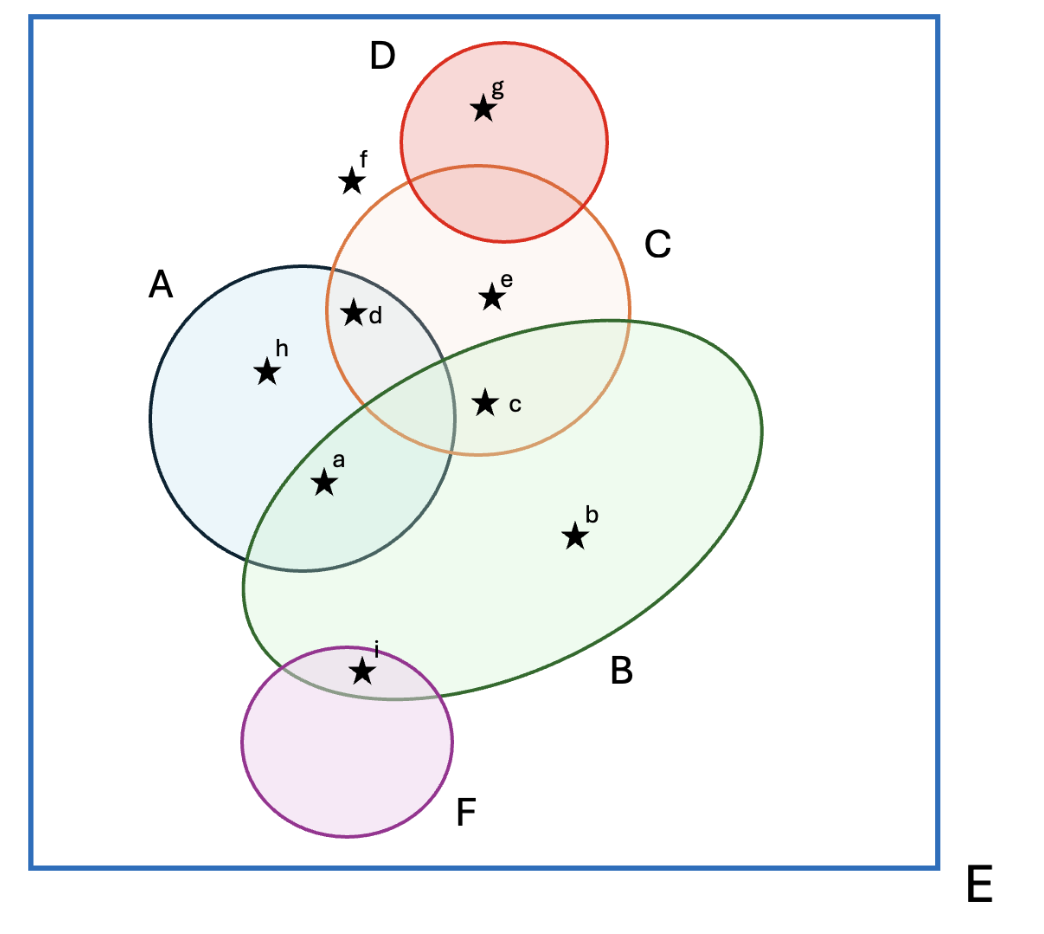
\includegraphics[width=0.6\textwidth]{img/venn.png}
\end{center}


Parmi les assertions suivantes, lesquelles sont correctes? (Plusieurs réponses possibles)

\mcqlist{
    {$d \in (A \cap C) \setminus D$},
    {$c \in (A \cup D) \cap B$},
    {$g \in \overline{A \cup B \cup C}$},
    {$f \in (D \cup C) \cap \overline{A \cup B \cup F}$},
    {$i \in \left(F \cap B \cap \overline{A \cup C \cup D}\right)$},
    {$\{c,e\} \subset (B \cap C) \cup (C \cap D)$},
    {$\{a,i\} \subset B \cap F$},
    {$\{b,c,g\} \subset B \cup D$},
    {
        $\{a,h,i\} \subset (A \cup F) \setminus (C \cap B)$
    }
}
\begin{solution}
Options: A, C, E, H, I. 
\end{solution}

\end{Exercice}

\begin{Exercice}[5 minutes]\textbf{Aurore}
Combien de sous-ensembles contient l'ensemble E = \{1,2,3,4\}?

\mcqlist{
    4, 8, 16, 32
}

\begin{solution}
Option C. Pour un ensemble de $n$ éléments, le nombre de sous-ensembles est donné par $2^n$.
\end{solution}

\end{Exercice}

\begin{Exercice}[5 minutes]\textbf{Aurore}
Dans lesquels des cas suivants la proposition suivante est-elle vraie?
$$
\bigl(((P \land Q) \lor P) \land (\lnot Q \land Q)\bigr)
\lor (\lnot P \land Q)
\lor (P \lor Q)
$$

\mcqlist{
    {$P=V,Q=V$},
    {$P=V,Q=F$},
    {$P=F,Q=V$},
    {$P=F,Q=F$},
    {Aucune de ces réponses n'est correcte}
}

\begin{solution}
A, B, et C.
\end{solution}

\end{Exercice}

\begin{Exercice}[5 minutes]\textbf{Aurore}
Laquelle de ces propositions est vraie par rapport à la classe Java qui débute par la ligne de code suivante:

\lstinline[style=javastyle]{public abstract class Country}
\mcqlist{
    {Elle s'agit d'une interface},
    {Elle peut être instanciée},
    {Elle peut hériter d'une autre classe si le nom est suivi du mot-clé implements},
    {Elle peut contenir des méthodes abstraites},
}

\begin{solution}
Option D. 
\end{solution}

\end{Exercice}

\pagebreak
\section{Algorithmes et complexité}


\begin{Exercice}[5 minutes]\textbf{Maxim}
Soit le code suivant. Quelle est sa complexité?

\begin{lstlisting}[style=pythonstyle]
def boucle(n):
    k = 0
    for i in range(n):
        for j in range(100):
            k += 1
    return k
\end{lstlisting}

\mcqlist{
 $O(\log n)$,
 $O(n)$,
 $O(n^2)$,
 $O(1)$
}

\begin{solution}
$O(n)$
\end{solution}

\end{Exercice}


\begin{Exercice}[5 minutes]\textbf{Maxim}
Soit le code suivant. Quelle est sa complexité?

\begin{lstlisting}[style=pythonstyle]
def boucle(n):
    k = 0
    for i in range(n):
        for j in range(i):
            k += 1
    return k
\end{lstlisting}

\mcqlist{
 $O(n^2)$,
 $O(n)$,
 $O(n\cdot \log n)$,
 $O(\log n)$
}

\begin{solution}
$O(n^2)$
\end{solution}

\end{Exercice}


\begin{Exercice}[5 minutes]\textbf{Maxim}
Soit le code suivant. Quelle est sa complexité?

\begin{lstlisting}[style=pythonstyle]
i = 1
while i < n:
    for j in range(n):
        print(i, j)
    i = i * 2
\end{lstlisting}

\mcqlist{
 $O(n^2)$,
 $O(n)$,
 $O(n\cdot \log n)$,
 $O(\log n)$
}

\begin{solution}
$O(n\cdot \log n)$
\end{solution}

\end{Exercice}

\begin{Exercice}[5 minutes]\textbf{Aurore}
Quelle est la complexité de la fonction suivante?

\begin{lstlisting}[style=javastyle]
public static void fonction(String word,int m) {
   int n = word.length()-1;
   while (n >= 0) {
       for (int i=0;i<m;i++) {
           System.out.println(word.charAt(n));
       }
       n--;
   }
}
\end{lstlisting}

\mcqlist{
    $O(n)$,
    $O(n^2)$,
    $O(n\cdot m)$,
    $O(n+m)$
}

\begin{solution}
$O(n\cdot m)$
\end{solution}

\end{Exercice}

\begin{Exercice}[5 minutes]\textbf{Aurore}
En applicant la fonction \textsc{mergeSort} telle que vue en cours sur la liste suivante, quelle est la paire de sous-listes sur laquelle merge() ne sera à aucun moment appelé [9,6,2,4,5,8]? 

\begin{lstlisting}[style=pythonstyle, caption={Merge sort — Python}]
def mergeSort(arr):
    if len(arr) <= 1:
        return arr
    
    mid = len(arr) // 2
    left = mergeSort(arr[:mid])
    right = mergeSort(arr[mid:])
    
    return merge(left, right)
\end{lstlisting}

\mcqlist{
    {$[6], [2]$},
    {$[2, 6, 9], [4, 5, 8]$},
    {$[4], [5, 8]$},
    {$[2], [4]$}
}

\begin{solution}
Option D: [2], [4]
\end{solution}
\end{Exercice}

% \begin{Exercice}[5 minutes]\textbf{Sean}

% Comment modifier tri-fusion pour que la liste soit triée par ordre décroissant:

% \mcqlist{
%     {Inverser la liste avant de commencer le tri.},
%     {Changer l'ordre des appels récursifs (traiter la partie droite avant la gauche)},
%     {Modifier le signe de comparaison dans l'étape de fusion.},
%     {Aucune de ces réponses}
% }

% \begin{solution}
% Option C.
% \end{solution}


% \end{Exercice}

\begin{Exercice}[5 minutes]\textbf{Sean}
Combien de fois la fonction \texttt{merge} va être appelée lors du tri-fusion sur une liste de $n$ éléments  

\mcqlist{
    $n$,
    $\log_2 n$,
    $n-1$,
    Cela dépend de la parité de la liste
}

\begin{solution}
Option C. Soit $f(n)$ la fonction qui donne le nombre d'appels à \texttt{merge}. On peut définir cette fonction récursivement suivant l'implémentation de \texttt{mergeSort}: $f(n) = 1 + 2\cdot f(\frac{n}{2})$. En remplaçant $f(n) = n-1$ on trouve que cette égalité est vraie. 
\end{solution}
\end{Exercice}

\begin{Exercice}[5 minutes]\textbf{Sean}
Quelle est la modification la plus efficace pour correctement supprimer les doublons de la liste pendant son tri avec l'algorithme de tri-fusion. 

\mcqlist{
    {Trier normalement, puis parcourir la liste finale pour retirer les éléments identiques.},
    {Vérifier si l'élément existe déjà dans la liste complète avant chaque insertion.},
    {Si les deux éléments comparés sont égaux dans \texttt{merge}, n'en ajouter qu'un seul au résultat et avancer les deux indices.},
    {Aucune de ces réponses}
}
\begin{solution}
Option C. 
\end{solution}
\end{Exercice}

\begin{Exercice}[5 minutes]\textbf{Léa}
Soient les affirmations suivantes:

\begin{itemize}
\item Si Alice prend un dessert, Bob en prend un aussi.
\item Chaque jour, soit Bob, soit Cathy, mais jamais les deux, prend un dessert.
\item Alice ou Cathy, ou les deux, prennent chaque jour un dessert.
\item Si Cathy prend un dessert, Alice fait de même.
\end{itemize}

Quelle combinaison de personnes prend un dessert si toutes les affirmations sont vraies?

\mcqlist{
    Alice seulement,
    Bob seulement,
    Cathy seulement,
    Alice et Bob uniquement
}

\begin{solution}
Option D: Alice et Bob uniquement. Cathy ne peut pas en prendre (car alors Alice et Bob devraient aussi, cela contredit soit Bob soit Cathy).
Donc Alice et Bob prennent un dessert.
\end{solution}

\end{Exercice}

\begin{Exercice}[5 minutes]\textbf{Léa}
Dans un ensemble E, considérons trois parties A, B, C. On sait que:

\begin{itemize}
\item $\{h, b\} \subset \overline{A} \cap \overline{B}$
\item $\{a, f\} \subset A \cup C$
\end{itemize}

Laquelle des propositions suivantes est vraie?

\mcqlist{
    {$h \in A$},
    {$b \in B$},
    {$a \in A \cup C$},
    {$f \notin C$}
}

\begin{solution}
$a \in A \cup C$.
\end{solution}

\end{Exercice}

\begin{Exercice}[5 minutes]\textbf{Léa}
Lesquelles des affirmations suivantes sont vraies concernant une classe abstraite Java.

\mcqlist{
    Peut être instanciée directement,
    Doit obligatoirement contenir au moins une méthode abstraite,
    Peut contenir des méthodes abstraites ou non,
    Ne peut pas contenir d’attributs
}

\begin{solution}
Option C. Une classe abstraite peut avoir zéro ou plusieurs méthodes abstraites, et des méthodes classiques.
\end{solution}

\end{Exercice}

\begin{Exercice}[5 minutes]\textbf{Léa}
Lesquelles des affirmations suivantes sont vraies concernant une interface Java.

\mcqlist{
    Les méthodes sont private par défaut,
    Les méthodes sont public abstract par défaut,
    Les variables sont privées par défaut,
    Les variables ne peuvent pas être finales
}

\begin{solution}
Option B. Les méthodes sont public abstract par défaut.
\end{solution}

\end{Exercice}

\begin{Exercice}[5 minutes]\textbf{Léa}
Quelle est la séquence correcte d’étapes du tri fusion?

\mcqlist{
        {
        Fusionner toute la liste \newline
        Diviser en deux moitiés \newline
        Trier séparément \newline
        Arrêter
    },
    {
        Diviser la liste en deux moitiés \newline
        Diviser encore chaque moitié jusqu’à obtenir des listes de taille 1 \newline
        Fusionner les petites listes pour former des listes triées \newline 
        Continuer les fusions jusqu’à obtenir une seule liste triée \newline
    },
    {
        Trouver le plus petit élément \newline
        Le placer au début \newline
        Répéter pour le second plus petit, etc. \newline
        Arrêter
    },
    {
        Trier d’abord la moitié droite \newline
        Trier ensuite la moitié gauche \newline
        Coller les deux moitiés sans les comparer \newline
        Arrêter
    }
}

\begin{solution}
Option B. 
\end{solution}

\end{Exercice}

\begin{Exercice}[5 minutes]\textbf{Léa}
Quelle est la complexité du code suivant supposant que la liste \texttt{L} contient $n$ éléments?

\begin{lstlisting}[style=pythonstyle]
def multiply(L):
    total = 1
    for x in L:
        total = total * x
    return total
\end{lstlisting}

\mcqlist{
    $O(1)$, $O(\log n)$, $O(n)$, $O(n^2)$
}


\begin{solution}
$O(n)$. 
\end{solution}

\end{Exercice}

\begin{Exercice}[5 minutes]\textbf{Maxim}

Quelle condition impérative une collection doit-elle respecter pour qu'on puisse y appliquer une recherche binaire (Binary Search)?

\mcqlist{
    Elle doit être triée., Elle doit être stockée dans une liste chaînée., Elle ne doit pas contenir de doublons., Elle doit contenir uniquement des entiers.
}

\begin{solution}
Option A. 
\end{solution}
\end{Exercice}

\begin{Exercice}[5 minutes]\textbf{Maxim}

Soit un arbre de recherche binaire vide dans lequel on insère la séquence suivante : {47,23,89,11,37,73,97}. Si on insère ensuite la valeur 31, où atterrit-elle?

\begin{center}

\includegraphics[width=0.6\textwidth]{img/tree.png}
\end{center}

\mcqlist{
    Comme enfant droit de 11., Comme enfant gauche de 73., Comme enfant gauche de 37., Comme enfant droit de 23.    
}

\begin{solution}
Option C. 
\end{solution}
\end{Exercice}

\begin{Exercice}[5 minutes]\textbf{Amina}
Soit la fonction suivante qui vérifie si une chaîne de caractères est un palindrome. Quelle est sa complexité temporelle supposant que la longueur de la chaîne de caractères est $n$?

\begin{lstlisting}[style=pythonstyle]
def est_palindrome(chaine: str) -> bool:
    chaine_nettoyee = "".join(filter(str.isalnum, chaine.lower()))
    n = len(chaine_nettoyee)
    
    gauche = 0
    droite = n - 1
    
    while gauche < droite:
        if chaine_nettoyee[gauche] != chaine_nettoyee[droite]:
            return False
            
        gauche += 1
        droite -= 1
        
    return True
\end{lstlisting}

\mcqlist{
    $O(n)$,  $O(n \log(n)$,  $O(1)$, $O(n^2)$
}

\begin{solution}
$O(n)$
\end{solution}

\end{Exercice}

\begin{Exercice}[5 minutes]\textbf{Amina}
Quelle notation asymptotique donne une borne supérieure asymptotique pour une fonction $f(n)$?


\mcqlist{
     $\Omega$-notation ,  $\Theta$-notation,  $O$-notation, $n_0$-notation
}

\begin{solution}
$O$-notation
\end{solution}

\end{Exercice}

\begin{Exercice}[5 minutes]\textbf{Sean}
Quelles affirmations sont correctes concernant les graphes denses?

\mcqlist{
    Un graphe complet est un graphe dense.,
    Un graphe connecté est un graphe dense.,
    Les listes d'adjacence sont plus efficaces pour représenter des graphes denses.,
    Les matrices d'adjacence sont plus efficaces pour représenter des graphes denses.
}

\begin{solution}
A, D.
\end{solution}
\end{Exercice}


\begin{Exercice}[5 minutes]\textbf{Sean}
Lesquelles des affirmations suivantes concernant l'algorithme de Kruskal sont vraies?

\mcqlist{
    L'algorithme de Kruskal utilise une approche gloutonne pour trouver l'arbre couvrant de poids minimal.,
    L'algorithme de Kruskal fonctionne aussi avec des poids négatifs.,
    L'algorithme de Krusal fonctionne sur des graphes non-connectés.,
     L'algorithme de Kruskal trouve l'unique solution optimale pour le problème de l'arbre couvrant de poids minimal.
}

\begin{solution}
B, E.
\end{solution}
\end{Exercice}

\begin{Exercice}[5 minutes]\textbf{Sean}
Lesquelles des affirmations suivantes concernant l'algorithme de parcours en largeur (BFS) sont vraies?

\mcqlist{
    L'algorithme BFS peut être utilisé pour trouver le plus court chemin dans un graphe non pondéré.,
    L'algorithme BFS utilise une pile (stack) pour garder la trace des nœuds à visiter.,
    {L'algorithme BFS visite tous les nœuds à une distance donnée avant de visiter les nœuds à la distance supérieure.},
    {Si il n'existe pas de chemin entre le nœud de départ et un autre nœud, l'algorithme BFS peut entrer dans une boucle infinie.},
    {Si le graphe contient des cycles, l'algorithme BFS ne peut pas être utilisé pour trouver le plus court chemin}.
}

\begin{solution}
A, C.
\end{solution}
\end{Exercice}

\begin{Exercice}[5 minutes]\textbf{Sean}
Combien d'appels à \textsc{UNION} sont nécessaires pour fusionner n ensembles disjoints en un seul ensemble?

\mcqlist{
    $n$,
    $n - 1$,
    $n + 1$,
    $2n$
}

\begin{solution}
Option B. L'arbre minimum couvrant a toujours $n-1$ arêtes pour $n$ sommets. Chaque appel à \textsc{UNION} crée une arête.  
\end{solution}
\end{Exercice}

%% TODO: Add Reda's questions here 

\begin{Exercice}[5 minutes]\textbf{Léa}
On applique une recherche séquentielle sur la liste \texttt{L = [5, 12, 7, 12, 20]} et on cherche 12.

Que renvoie l’algorithme de recherche séquentielle suivant?

\begin{lstlisting}[style=pythonstyle]
def recherche_sequentielle(liste, e):
    if e in liste:
        return liste.index(e)
    return -1 
\end{lstlisting}

\mcqlist{
1, 3, 12, (1, 3)
}

\begin{solution}
1
\end{solution}


\end{Exercice}


\begin{Exercice}[5 minutes]\textbf{Léa}
On cherche \texttt{key = 11} dans la liste triée \texttt{L = [2, 4, 6, 10, 13, 18]}. Que renvoie l'algorithme de recherche binaire suivant?

\begin{lstlisting}[style=pythonstyle]
def recherche_binaire(key, array):
    low = 0
    high = len(array) - 1

    while low <= high:
        mid = (low + high) // 2

        if key < array[mid]:
            high = mid - 1
        elif key > array[mid]:
            low = mid + 1
        else:
            return mid

    return -1
\end{lstlisting}

\mcqlist{
3, KeyError: 11, -1, 11
}

\begin{solution}
-1
\end{solution}

\end{Exercice}


\begin{Exercice}[5 minutes]\textbf{Léa}
On considère le graphe suivant, représenté par une liste d’adjacence:

\begin{lstlisting}
G = {
   'A': ['B','D'],
   'B': ['C'],
   'C': ['E'],
   'D': ['E'],
   'E': []
}
\end{lstlisting}

L'algorithme de BFS: 

\begin{lstlisting}[style=pythonstyle]
def bfs(graph, start):
    visited = list(start) # liste des sommets visités
    queue = [start] # liste des sommets à visiter
    order = [] # pour stocker l'ordre de sommets
    u = queue.pop(0) 
    order.append(u)
    neighbors = graph[u] # liste des voisins de u
    for v in neighbors : 
        if v not in visited : 
            queue.append(v)
            visited.append(v)
return order 
\end{lstlisting}

Que retourne \texttt{BFS(G, 'A')}?

\mcqlist{
{$[$'A','B','D','C','E'$]$ }, {$[$'A','D','B','C','E'$]$}, {$[$'A','B','C','D','E'$]$}, {$[$'A','D','E','B','C'$]$}
}

\begin{solution}
Option A. 
\end{solution}

\end{Exercice}

\begin{Exercice}[5 minutes]\textbf{Léa}
Soit le graphe décrit par la liste d'adjacence (adjacency list) ci-dessous:

\begin{lstlisting}
G = {
  "A": [("B", 3), ("C", 1)],
  "B": [("A", 3), ("C", 2), ("D", 4)],
  "C": [("A", 1), ("B", 2), ("D", 5)],
  "D": [("B", 4), ("C", 5)]
}
\end{lstlisting}

Quel ensemble d’arêtes forme l’arbre couvrant minimal obtenu avec Kruskal?

\mcqlist{
{('A','C',1), ('B','C',2), ('B','D',4)},
 {('A','C',1), ('A','B',3), ('B','D',4)},
 {('A','C',1), ('B','C',2), ('A','B',3)},
{('A','B',3), ('B','C',2), ('C','D',4)}
}

\begin{solution}
Option A. 
\end{solution}

\end{Exercice}



\begin{Exercice}[5 minutes]\textbf{Sean}
Soit l'algorithme de construction d'un arbre KD (KD-tree) avec $K=3$, et un ensemble de points en 3D sous la forme $(x, y, z)$.
Si le premier axe de division est l'axe $X$, le deuxième $Y$ et le troisième $Z$, quel axe sera utilisé lors du troisième appel à \textsc{BuildKDTree} étant donné qu'il y a 10 points distincts?

\begin{algorithm}[H]
\caption{BuildKDTree($\text{points}, \text{depth}, k$)}
\label{alg:kdtree-build}
\begin{algorithmic}[1]
\If{$\text{points} = \emptyset$}
    \State \textbf{return} $\text{NIL}$
\EndIf
\State $\text{axis} \leftarrow \text{depth} \ \% \ k$ \Comment{Select axis based on current depth}
\State $\text{points} \leftarrow \text{SORT}(\text{points}, \text{key} = \text{axis})$ \Comment{Sort by current axis}
\State $\text{median\_idx} \leftarrow \text{INTEGER}(\text{length}(\text{points}) / 2 )$ \Comment{Index of median list item}
\State $\text{median} \leftarrow \text{KDNode}(\text{points}[\text{median\_idx}]$)
\State $\text{left} \leftarrow \text{points}[1 \ldots \text{median\_idx} - 1]$ \Comment{Left half of the points list}
\State $\text{right} \leftarrow \text{points}[\text{median\_idx} + 1 \ldots \text{length}(\text{points})]$ \Comment{Right half of the points list}
\State $\text{median.left} \leftarrow \text{BuildKDTree}(\text{left}, \text{depth} + 1, k)$
\State $\text{median.right} \leftarrow \text{BuildKDTree}(\text{right}, \text{depth} + 1, k)$
\State \textbf{return} median
\end{algorithmic}
\end{algorithm}

\mcqlist{
    X, Y, Z
}

\begin{solution}
Z
\end{solution}

\end{Exercice}

\begin{Exercice}[5 minutes]\textbf{Sean}
Lesquelles des affirmations suivantes concernant les quadtrees sont vraies?

\mcqlist{
    {Les Quadtrees sont toujours des arbres équilibrés.},
    {Chaque nœud interne d'un Quadtree a exactement quatre enfants.},
    {Les Quadtrees sont principalement utilisés pour représenter des données en trois dimensions.},
    {Avec une profondeur de $n$ (hauteur de l'arbre), un Quadtree peut représenter jusqu'à $2^n$ régions distinctes.},
    {Avec une profondeur de $n$ (hauteur de l'arbre), un Quadtree peut représenter jusqu'à $4^n$ régions distinctes. }
}

\begin{solution}
B, E. 
\end{solution}
 

\end{Exercice}



\begin{Exercice}[5 minutes]\textbf{Aurore}
Laquelle des affirmations suivantes est fausse concernant les algorithmes de recherche?

\mcqlist{
    {La complexité d'un algorithme de recherche binaire est de O(log(n)).},
    {La performance de la recherche binaire est meilleure que celle de la recherche séquentielle pour de grandes collections.},
    {La recherche par arbre de recherche binaire est une recherche dichotomique.},
    {La recherche séquentielle requiert une collection triée.},
    {Toutes les affirmations sont correctes. }
}
\begin{solution}
Option D. 
\end{solution}


\end{Exercice}




\end{document}
